%Copyright (C) 2021  Geoff Beck
%
%This document is falls under the category of free software: you can redistribute it and/or modify
%it under the terms of the GNU General Public License as published by
%the Free Software Foundation, either version 3 of the License, or
%(at your option) any later version.
%
%This program is distributed in the hope that it will be useful,
%but WITHOUT ANY WARRANTY; without even the implied warranty of
%MERCHANTABILITY or FITNESS FOR A PARTICULAR PURPOSE.  See the
%GNU General Public License for more details.
%
%See https://www.gnu.org/licenses/ for more details

\documentclass[a4paper,10pt,oneside]{book}

\usepackage{fullpage}
\usepackage{amsmath}
\usepackage{import,url}
\usepackage{tocbibind}
\usepackage[bookmarks=true,plainpages=false]{hyperref}
\usepackage{titletoc}
\usepackage{graphicx}
\usepackage{caption,titlecaps}
\usepackage[a4paper,margin=2cm]{geometry}

\graphicspath{{pictures/}}
\usepackage[T1]{fontenc}
\usepackage{lmodern}


\subimport{../}{dice}

\newcommand{\textlf}[1]{\textbf{\titlecap{#1}}}
\newcommand{\textlfirst}[1]{\textbf{\textit{\titlecap{#1}}}}

\title{\textbf{\huge 3d6 Heroes \\Core Rules \\Version 10.1}}
\author{Geoff Beck}
\date{}

\begin{document}
\maketitle
\frontmatter
\tableofcontents
\mainmatter

\chapter{Introduction}

\section{Opening Words}
A player's character is their representative in the world of \textit{Heroes} and such should be a personal and fully customisable thing; allowing the player's creativity free reign and not limiting him with too many rules and class attributes etc. This is what \textit{Heroes} tries to do, liberate your role playing experience from restrictive parameters but still maintain some semblance of an ordered and enjoyable system.

\textit{Heroes} depends almost as much on the imagination of the players as it does upon the Game Master. The players are given little or no instruction as to how to fulfil any role within a group and how well they do this will ultimately decide how much fun the game is.

This is a simple system to pick up, as it applies a central set of mechanics across the board, but is complicated enough to please even the most hardcore of gamers, due to the depth and freedom of its mechanics, should you choose to delve into them. The system itself is very open to interpretation and lots of work is required by the Game Master to make this work, as he must make many decisions on the spot as to how he will apply rules to a given situation. Other than that, just read and play.

This weighty tome encompasses all the essential rules needed to play a game of \textit{Heroes} independent of setting, other books merely contain rules for playing the game within a famous/iconic world or setting, all these other books require these Core Rules, but do occasionally over-ride them when necessary.

This rule book falls under the category of free software~\footnote{Copyright (C) 2021  Geoff Beck}: you can redistribute it and/or modify
it under the terms of the GNU General Public License as published by
the Free Software Foundation, either version 3 of the License, or any later version (see \url{https://www.gnu.org/licenses/}).

\section{The Core System}
\label{sec:base}

\subsection{Players and the Game Master (GM)}
Games of Heroes are run by a player designated as the Game Master (GM). The remaining participants are simply termed as players. Each of the players controls a character and together they will take part in an adventure supervised by the GM. The Game Master acts as a narrator, he drives the story and is in control of the world and environments inhabited by the player characters. Additionally, he creates and controls any people or monsters that the characters will encounter in the course of their adventures. 

These rules for the structure of the game are deliberately loose, as the freedom of players and GM to collectively shape an adventure is the magic that makes pen-and-paper role-playing games worthwhile.

\subsection{Actions and Dice Rolls}
An element of randomisation is introduced into the game by the players rolling dice whenever their characters wish to perform non-trivial actions. These rolls tend to be modified by how good the character is at the particular action (making him more or less likely to succeed). Things like breaking down doors, persuading a guard to let you into a locked door, picking a lock, fighting an enemy, noticing someone hiding in the bushes, climbing a tree/wall/ladder/rope, swimming, jumping a gap, riding, or picking pockets are all examples of actions that would require the player to make a roll to see if his character succeeds. 

How good a character is at a particular action is decided by two things, firstly his natural capabilities (Chapter~\ref{chap:attb}) and secondly his learned or acquired skills (Chapter~\ref{chap:skills}). Deciding whether or not a skill or natural attribute is appropriate to a particular task is a matter of common sense and the players and GM can come to a consensus for any contentious tasks. For example: tasks that rely only on the characters strength (actions like breaking things) will not be resolved through skills. However, actions like riding horses, tying or climbing ropes, and picking locks are all things that are greatly enhanced by experience and skill development and thus will rely on skills when resolving such actions. Note that skills still benefit from natural attributes, usually those that give one some advantage in the particular discipline. 

How success and failure are determined is explained in the Section~\ref{sec:rolls} below.

\subsubsection{Dice Notation}
The notation ``requires a 3d6 roll of 16+" means that a total score of 16 or greater, on three six-sided dice (3d6), is needed for the given action to succeed. Similarly ``5-" means 5 or less. When no dice code (3d6, 2d6, etc) is given, then 3d6 is considered the default dice set.

\subsubsection{Roll Descriptors}
A score that is described as being \textlfirst{raw} or \textlfirst{unmodified}, is one that is directly generated by a set of dice, prior to the application of any numerical modification. A modified score is a one that is generated by a set of dice and then has some bonus or penalty applied to it to generate a final score.

\subsubsection{The Opposed Roll and Difficulty Check}
\label{sec:rolls}
The core of this 3d6 system is the \textlfirst{difficulty check}, any task can be assigned a \textlfirst{difficulty} by the Game Master and then is performed successfully if the character scores equal to or greater than the \textlf{difficulty} on a roll of 3d6. To this roll you add the relevant \textlfirst{attribute/skill} score; for instance when making a climbing check you add your athletics score to the roll. The second core mechanic is the \textlfirst{opposed roll}, this represents a contest between two or more opponents, as such each creature contesting the roll adds the given \textlf{attribute/skill} score to a roll of 3d6. The victor is the one whose resultant score is the highest. In the case of a tie, simply roll again.

%\subsubsection{Success and Failure}
%The threshold for success on 3d6 is exceeding the task \textlf{difficulty} after applying any score modifiers. %However, if the raw score is $\dicefail-$ then the action is always a failure regardless of modifiers (this is referred to as \textlfirst{total failure}). If the raw score is $\dicecritical+$ then the action always succeeds regardless of modifiers.

\subsubsection{Critical Success/Failure}
If you succeed/fail on a check by $\dicecritlvl$ or more you have achieved a \textlfirst{critical success/failure}. For example if you need to beat \textlf{difficulty} 11 to succeed then 16 is \textlf{critical success} whereas 6 is \textlf{critical failure}. Some effects scale with how many multiples of $\dicecritlvl$ you succeed or fail by.

\subsubsection{Rounding Conventions}
When the division of an integer score results in a non-integer number (i.e. it is not a whole number) then the convention is to round up. Unless otherwise specified.

\subsubsection{Edge}
Some circumstances confer great advantage or disadvantage on a character. This is referred to as \textlfirst{edge}. While experiencing an \textlf{edge} bonus on a roll, a character makes the roll twice and chooses the higher score. In contrast, an \textlf{edge} penalty makes the character roll twice and choose the lower score. 

An \textlf{edge} penalty cancels out a bonus if character is subject to both. If a character has 2 or more \textlf{edge} bonuses/penalties simply add an extra roll to the pool (so 2 \textlf{edge} bonuses means roll 3 sets of dice and choose the highest etc).

\subsection{Heroic Statistics}
Any heroic/villainous character will also posses an attribute called \textlfirst{heroism/villainy}, which can be spent to perform feats of exceptional skill and daring. The central premise of this statistic system is to set heroic characters apart, as the feats performed through the use of heroism points must be formulated by the players themselves (with the Game Master moderating their effects). Players are encouraged, then, to be creative, outrageous, and down-right crazy in their use of these abilities, the laws of physics are, here, less important than stylish, action-packed adventure.




\chapter{Character Attributes}
\label{chap:attb}

A character in \textit{Heroes} is represented by a set of \textlfirst{natural attributes} and their \textlf{heroism/villainy}. The former detail the character's innate abilities while the latter represent his calibre as a potential hero or villain.
Natural attributes are: \textlfirst{might}, \textlfirst{cunning}, \textlfirst{perception}, and \textlfirst{resolve}.%, and \textlfirst{agility}.

Natural attributes can be used to determine a character's success in certain actions (examples are given in the sections below). As such, success is determined by making a \textlf{difficulty check} with the given attribute.

\section{Natural Attributes}
These reflect the inherent predispositions of the character, based on their personality. There are five attribute statistics and a character's scores are determined following the character creation rules, found in Chapter~\ref{chap:create}. 

\subsection{Attribute Modifiers}
Each attribute contributes to many different skills or activities, its influence on dice rolls is direct, just add it to the result of a relevant roll.

\subsection{Might}
\textlf{Might} is the physical/spiritual power and aggressiveness of the character. A character can make might-checks to break objects through sheer force or determination, to bash in doors or to move large objects. The \textlf{difficulty} of breaking objects can be found under the rules for \textlf{Cover}, Section~\ref{sec:cover}, in the Combat rules.\textlf{Difficulty} for lifting or moving heavy objects can be found in Section~\ref{sec:carry} in Baggage and Encumbrance. \textlf{Might} also dictates a character's ability to inflict damage in combat.

%Characters with \textlf{might} scores of 0 tend to be more peaceful, while less than -2 means that the character struggles to bring himself to inflict harm. \textlf{Might} 0 or greater represents a forceful and aggressive character, with scores between 3 and 5 verging on superhuman ferocity.

\subsection{Cunning}
\textlf{Cunning} is the craftiness of the character. \textlf{Cunning} checks can be used to bluff convincingly, make feints in combat, or get out of the way of harm. \textlf{Cunning} contributes to the \textlf{stealth}, \textlf{disguise}, \textlf{deceive}, \textlf{slight of hand}, \textlf{survival}, and \textlf{mechanical} skills. \textlf{Cunning} also influences the power of a character's underhanded manoeuvres in combat, such as \textlf{sneak attacks} or back-stabbing.

%Characters with low \textlf{cunning} (less than -1) are not very devious and tend to be honest and ingenuous. Very low scores might mean that the character is just too trusting, verging on idiocy in his lack of caution. \textlf{Cunning} of 0 or greater means the character can be sly and crafty, with scores of 3 or more indicating that the character has the makings of a master plotter..

\subsection{Perception}
\textlf{Perception} is a character's ability to spot/analyse details, as such it involved in the \textlf{shooting}, \textlf{close-combat}, and \textlf{awareness} skills. \textlf{Perception} also contributes to a character's ability to cast spells or use/activate similar occult abilities. \textlf{Perception} checks are necessary to making rapid decisions in high pressure situations (like choosing a key from a large bunch to escape a room that is filling with water). The \textlf{difficulty} of such checks is given by how imminent the danger is. \textlf{Perception} also decides how difficult it is to deceive or confuse the character. 

%Characters with scores below -1 are quite oblivious and carefree. Those with \textlf{Perception} below -2 are almost entirely unaware of their surroundings. Scores of 0 or greater imply that the character is attentive and shrewd, with \textlf{Perception} scores of 3 or above meaning they are unlikely to miss even the smallest detail.

\subsection{Resolve}
Is a measure of the character's determination and force of character. \textlf{Resolve} checks can be used to flatter, distract, or to taunt/enrage a target into attacking the character. The \textlf{difficulty} of such checks is given by the target's \textlf{perception} score. Such a check might also be made to subtly get someone talking to you, the \textlf{difficulty} is dictated by how reticent or secretive they are (this is indirect unlike a \textlf{persuade} attempt). \textlf{Resolve} is also involved in the \textlf{persuade}, \textlf{leadership}, and \textlf{perform} skills. Additionally, it regulates a character's ability to resist debilitating effects (magic,drugs,poisons) by pure will. 

%Characters with low \textlf{resolve} (less than -1) are either spineless or just socially awkward. Very low scores (less than -2) imply that the character can hardly communicate for shyness, is just impossible to tolerate, or hopelessly easy to bully. \textlf{Resolve} of 0 or greater makes for a compelling or attractive character, with scores of 3 or greater indicating a force of personality, or charm, that sweeps others along with it. 

%\subsection{Agility}
%\textlf{Agility} is the character's reaction speed and general coordination. \textlf{Agility} checks can be made to execute sudden moves, like grabbing for a weapon being pointed at you or ducking for cover from an explosion. \textlf{Agility} determines a character's ability to evade harmful attacks or effects, contributes to the speed with which he makes his actions in combat, and influences the \textlf{ride} and \textlf{athletics} skills.
%
%Characters with low \textlf{agility} (less than -1) are slightly slow and clumsy. Very low scores might mean that the character is likely to trip over his own feet while crossing the room. \textlf{Agility} of 0 or greater means the character is very swift and dexterous, moving with grace and being capable with both hands and feet, with scores of 3 or greater being indicative of fantastically fast reflexes and unparalleled sureness of movement. 

%\subsection{Fortitude}
%This represents a character's mental and physical toughness. A Fortitude check can be made to prevent a character being incapacitated by his Wounds. If he has suffered enough Wounds to knock him out he must pass a check with difficulty 10 each round, this goes up by 1 for each subsequent Wound suffered. Fortitude checks are also necessary to resist the ill effects of poisons, drugs and even magic (each of these effects will have a built-in difficulty). Fortitude also influences the Survival skill.
%
%Characters with low Fortitude (less than 8) are vulnerable, being physically or mentally frail. Very low scores might mean that the character is extremely weak and frightened of harm, he is probably a coward as well. Fortitude of 9 or greater means the character is highly durable, being strong of body or mind (or both), with scores of 12 or above represent superhuman resilience.



\section{Heroic Attributes}
\label{sec:heroism}
\subsection{Heroism/Villainy}
\textlf{Heroism} is what sets your character apart from his more ordinary brethren, it represents a hero's capacity to make decisive and daring actions under pressure. The distinction between \textlf{heroism} and \textlf{villainy} points is one of flavour, villains have \textlf{villainy} while heroes get \textlf{heroism}. Generally, if a rule refers to \textlf{heroism} it still pertains to \textlf{villainy}, unless otherwise stated. 

\textlf{Heroism/Villainy} may be spent to raise the critical success level of a single successful action by (i.e. a success become a critical success and critical success becomes a level 2 critical success). Additionally \textlf{heroism} may be spent to perform daring feats of valour while \textlf{villainy} may be used for vile trickery; this allows the character to make special actions he invents on the spot. The Game Master must decide the consequences of any such actions made. If a character has no \textlf{heroism/villainy} when he rests he may regain 1 point, otherwise such points are awarded by the Game Master on the spur of the moment for any deed that is appropriately heroic/villainous.


\subsubsection{Moment of Glory}
A \textlfirst{moment of glory} awards the character with a single \textlf{heroism/villainy} point he can spend within the next round only.


\section{Perks \& proficiencies}

\textlfirst{Perks} are talents learned or gained by a hero through the course of his adventures, they can be purchased via the expenditure of experience points. A character can have at most 3 active and 3 passive \textlf{perks} equipped ones at once (only equipped \textlf{perks} can be used). If they know more than 3, they may choose which 3 are active. Changing the active selection requires an hours rest and concentration.
\textlf{Proficiencies} are more general skills gained by the character. These are always active and never occupy either passive or active \textlf{perk} equipment slots.
A list of \textlf{perks} and \textlf{proficiencies} can be found in Chapter~\ref{chap:perks}.

\section{Experience points}
Each time the Game Master decides to reward the heroic achievement of a character, or each character in the group, then the relevant characters gain 1 experience point. 
This guideline is very qualitative and this is because heroism is a qualitative thing, so advancement is very much a case of the application of GM judgement, informed by basic guidelines laid down here.

Simple guidelines for experience: a point can be earned by actions demonstrating some heroic calibre, such as: single handedly over-coming many foes or performing reckless feats of strength and daring that save the day. Or perhaps by feats of magic or deeds accomplished through strength of will and force of personality (see also Section~\ref{sec:skill-adv}). Experience can also be awarded for devious acts of deceit, or from victory through wit and intelligence rather than blade and boot. Note that these achievements are not combat exclusive, heroism is format-independent after all.

Experience points can be spent on purchasing new \textlf{perks} and \textlf{proficiencies}, the costs of these is detailed in Chapter \ref{chap:perks}. 

%Natural attribute points can also be increased through the expenditure of experience, costing a number of points equal to the difference between the next level and 0 (or the current level and 0 if the next level is 0 or lower), multiplied by 5. Therefore increasing from -1 to 0 or from 0 to 1 costs 5, but from 1 to 2 costs 10 and 2 to 3 costs 15. 

Note that experience cannot be spent in high pressure or active situations, only during periods of rest and contemplation.

\subsection{Advancing Attributes}
Natural attribute points can  be increased through the expenditure of experience to a maximum of +3 for any given attribute. Advancement costs are shown in Table~\ref{tab:nat-att}. Note that to advance to level 2 you need to be level 1, etc. Therefore, the total cost of going from level 0 to 3 is 15 experience. 
\begin{table}[ht!]
	\centering
	\begin{tabular}{|c|c|}
		\hline
		Level & Cost \\
		\hline
		1 & 3 \\
		2 & 5 \\
		3 & 7 \\
		\hline
	\end{tabular}
	\caption{Natural attribute advancement table.}
	\label{tab:nat-att}
\end{table}  



\section{Reputation}
Any hero or villain has a reputation, be it as a magnanimous defender or a scheming thief; so to can characters develop a reputation and even, by great deeds, have their names known and talked of by thousands of admirers/policemen. 

\subsection{Reputation Level}
Reputation is gained by performing important deeds or actions that get you talked about. Saving the mayor's daughter or preventing orcs from killing a group of farmers, that kind of thing. Cheating lots of people out of their money or swindling a local lord or even robbing a bank are also good examples of reputation gaining actions.

Each character has a personal reputation, which is that of the group but modified by personal actions, and the group as a whole has a reputation based on group actions.

Characters start at 0 reputation.

\subsection{Reputation Rating}
This indicates whether your reputation is good or bad, it starts at 0 normally, but depending on your Game Master, it can start at -1 or +1. If you gain reputation for ``bad" actions you get -1 reputation rating, ``good" actions get +1, so a negative reputation makes you infamous while positive makes you well-liked.





\chapter{Making a Character}

\label{chap:create}
Simply follow these steps to create a character:
\begin{itemize}
\item
First browse the species available in the campaign setting and choose yourself a species, you may wish to select this based on the modifiers applied to members of that group, or simply on a whim.
\item
Now select a character \textlfirst{background} from \ref{sec:backgrounds}, or invent one your GM agrees to.
\item 
Select at least one \textlfirst{Conviction} for your character from \ref{sec:convictions} or invent your own.
\item
Select, or invent, the \textlfirst{Flaw} in your character's personality from \ref{sec:flaws} (you may select two at most).
\item
Decide the \textlfirst{goals} that drive your character to pursue adventure.
\item
What \textlfirst{relationships} link the character to other group members, organisations, or people in their past?
\item
Now we come to the most important part of character creation, deciding what kind of person your character is. Use the \textlf{Convictions}, \textlf{flaws} and \textlf{goals} you chose as a skeleton. You need to define a character you are comfortable to play as, but also one who is believable as a real person because, lets face it, its not much of a role playing game if everyone is just a faceless killing machine.
\item
Set all \textlf{attributes} to 0. You may then choose two \textlf{attributes} to elevate to +1.  Set \textlf{heroism/villainy} to 1. 
\item 
Spend up to 3 experience points choosing \textlf{perks} or \textlf{proficiencies} (Chapter~\ref{chap:perks}) for your character. All characters are proficient with light armour for free.
\item
A character must then choose 2 skills to be \textlf{proficient} in. These skills must be chosen from the ``associated skills" list for the character's background. 
\item
Now you may select starting equipment, either from a list supplied by the Game Master or from a budget.
\item
Calculate your combat statistics (see Section~\ref{sec:comstat}).
\end{itemize}



\section{Character backgrounds}
\label{sec:backgrounds}
The character's background is their history before adventuring and dictates the set of associated skills they can choose on character creation. Beyond selecting these you should also sketch out a brief back-story for the character, explaining how they fit into the chosen background archetype. You can, of course, add backgrounds appropriate to the setting.

\subsection{Soldier}
The character is a hard-bitten veteran of fighting. Having seen his fair share of blood spilt on the orders of others, he now turns his hand to adventuring instead. Soldier encompasses several possible histories: mercenaries, city guards, bandits, or gang enforcers. Associated skills: Close-combat, Shoot, Throw, Ride, Athletics, Leadership.

\subsection{Guttersnipe}
The character was born into a life of poverty, scrounging, stealing, and fighting for scraps in back-alleys. This background lends itself to a history that involves scavenging and surviving by any means necessary, street-smart characters who grew up in harsh environments. Such a character is used to being on the wrong side of the law, sometimes even through no fault of their own. Associated skills: Sneak \& Hide, Slight of hand, Deceive, Athletics, Awareness, Throw, Shoot.

\subsection{Wanderer}
The character lives the life of a vagrant or vagabond. He moves from place to place seeking opportunity, profit, or just thrills. However, many people are suspicious of such a lifestyle and regard the character with suspicion or outright hostility. Wanderer is suited to a character who likes wild places and is resentful or suspicious of petty authority. Associated skills: Survival, Shoot, Throw, Athletics, Sneak \& Hide, Awareness, Animals, Plants.

\subsection{Silver spoon}
The character was born into old money, nobility, or some similar high social station. They received an expensive education and live an expensive lifestyle. As such these characters are used to political manoeuvrings that go along with high society. Associated skills: Persuade, Deceive, Leadership, Ride, History, Religion, Shoot.

\subsection{Professional}
The character has trained long in a craft and has become quite skilled in his own right. This is a broad category and encompass scholars, blacksmiths, engineers, farmers, sailors, and many others. Associated skills: Mechanical, Profession skills, Awareness, Knowledge skills. 

\subsection{Artist}
The character has trained in the creative arts, being a musician/bard, actor, dancer, sculptor, painter or something similar. Such a character often has a near obsessive devotion to their art form and a tendency to grandiosity. Associated skills: Perform, Athletics, Persuade, Disguise, History, Religion, Throw.

\subsection{Barbarian}
The character is born into a culture deemed savage and backward by most civilised societies (civilisation is often in the eye of the beholder). Such `sophisticated' individuals therefore view him with a mixture of terror and revulsion. However, they have their own perspective on what it means to be civil and many valuable skills. Associated skills: Survival, Close-combat, Throw, Athletics, Awareness, Ride, Animal, Plant.



\section{Convictions}
\label{sec:convictions}
Convictions are your character's ideals and principles. Their moral code and the truths they believe in. These are suggestions and serve as a guideline for creating your own.

\subsection{Might makes right}
The character believes that strength justifies everything. The weak being preyed upon by the strong is just how the world works. 

\subsection{Nothing for nothing}
The character believes that everything has to be earned, charity only creates dependence.

\subsection{Something for nothing}
The character knows that the destitute need protection, mutual support strengthens everyone. The character believes strongly in charity and doing what they can to help anyone.

\subsection{Words before weapons}
The character will always try to talk before resorting to violence, they are a dedicated pacifist.

\subsection{Kill or be killed}
The character has no qualms about violence and resorts to it often, the non-violent don't last long enough for their principles to matter.

\subsection{Make your own justice}
The law is not be trusted, you have to claim justice for yourself rather than waiting for a court. 

\subsection{The law is the law}
Rules exist for a reason and should be obeyed as closely as possible.

\subsection{Power always corrupts}
No one can be trusted with power. All authority should be looked upon with suspicion as the powerful are the enemy.

\subsection{The ruled need rulers}
People are sheep and need a shepherd. Conveniently, you are just the person for the job.

\subsection{Serve a greater good}
There are things more important than any one individual, such a cause drives your actions (make up a suitable one).

\subsection{Knowledge is power}
Knowledge is vital, curiosity and the drive to learn are fundamental to civilisation. The character will always aim to ferret out secrets.

\subsection{Honour is paramount}
You cannot control how others behave but you can always choose to do the right thing. The character assiduously follows a code of honour (make up a suitable one).



\section{Flaws}
\label{sec:flaws}
Flaws are what make your character the imperfect creature they are. These are suggestions and serve as a guideline for creating your own.

\subsection{Jenkins}
The character is impulsive and will not hesitate to act while their comrades debate the best course of action.

\subsection{Clumsy}
The character is not the sharpest tool in the shed, in fact you will be lucky if they don't burn the shed down by accident while searching for tools.

\subsection{No Diplomat}
The character has a habit of saying the first thing to come into their head, regardless of how inappropriate it is to the current situation (they may not take the Diplomat power either).

\subsection{Dipsomaniac}
The character is a borderline addict to a chosen substance and will consume it whenever possible.

\subsection{All about Me}
Such a character will see themselves as the centre of events at all times and will seldom acknowledge the efforts and contributions of others. This can manifest in anything from a tendency to self-importance to a narcissistic view that any praise is their due and any criticism levelled against them is out of pure jealousy. 

\subsection{Better with Animals}
This character is a rough soul who prefers life in the thick of nature to a bustling city. As such they tend to be a bit brusque with ``soft" city dwellers and contemptuous of petty authorities like watchmen and mayors.

\subsection{In It to Win It}
The character takes competitive to the extreme, and has to be the best at everything they do. Their pride is greatly wounded when this is not the case. 

\subsection{Driven}
The character has a guiding obsession that they will seek to pursue regardless of more pressing matters.

\subsection{Scarred}
The character has been both mentally and physically scarred by exposure to violence or trauma. This may manifest as anything from flash-backs or violent outbursts to long boring stories about events of the character's past. The severity can be chosen based on the character's history.

\subsection{Out of Touch}
The character is absorbed in day dreams and speculation, often being more concerned with knowledge and thought than real events. As such, the character tends to appear forgetful and oblivious and can often cause touchy individuals to take offence (as they might feel ignored).

\subsection{Money grubber}
The character is greedy and always looks to profit regardless of the situation.

\subsection{Temper temper}
The character angers quickly and is prone to outbursts of anger when pushed.

\subsection{Arrogant}
The character is assured of their superiority to others and is often condescending.

\subsection{Paranoid}
The character sees a conspiracy in every shadow and a threat around every corner. They would sleep in full plate if they could.

\subsection{Too trusting} 
The character can't help but expect others to be as nice as they are. Thus, they implicitly trust everyone who doesn't seem outrageously shifty.

\subsection{Domineering}
The character is used to getting their own way. They don't take questioning of their authority well, expect everyone to do their bidding, and may be unwilling to listen to the ideas of others.

\subsection{Touchy}
The character has a sense of pride that can be easily bruised. They feel the need to have their usefulness affirmed often.

\subsection{Master debater}
The character can't help but argue. They will challenge any assertion they can and will pursue arguments relentlessly.



\section{Relationships}
\label{sec:relationships}
These are your character's links to other people or places, it is often sensible to select relationships that link your character to at least one other in the adventuring group. These can be things like old friends, family links, or an organisation that your character is part of or linked to. This can be a powerful tool for making your character a part of the world you adventure in, so it should be carefully considered.


\section{Goals}
\label{sec:goals}
Everyone has an ambition, something that motivates them to wake up every morning. Goals are what motivate your character to adventure. These can be things like fame, riches, public office, honours, or secret knowledge. Other suggestions could be revenge or the finding of lost friends/relatives. Think about choosing your goals as selecting an initial objective for your character, an opening arc to their story.




\chapter{Character Skills}
\label{chap:skills}
There are several skills available that allow characters to pursue a craft or profession outside of adventuring; as well as more general skills that might aid your progress through your adventures.

\section{Skill proficiency}
\label{sec:skill-prof}
If a character is \textlf{proficient} with a given skill then they add the synergy attribute to associated rolls. This attribute usually follows the skill name. Otherwise, they add -1. A character can either be trained in a skill (requires 20 hours of training) or spend 3 experience to gain proficiency.


\section{Using a Skill}
\label{sec:use-skill}
A skill check is made whenever it is deemed appropriate by the Game Master, for instance an athletics check must be made when a character wishes to jump over a precipice or to climb up a building. Further examples of when skills might be used are listed in their descriptions in following sections.

When using a skill the character must exceed the \textlf{difficulty} of the task on a roll of 3d6, adding either their synergy attribute or -1. The \textlf{difficulty} of a task is at the Game Master's discretion. If the roll equals or exceeds the required \textlf{difficulty} score, then a \textlfirst{success} is achieved. However, if the roll exceeds the \textlf{difficulty} by $\dicecritlvl$, or more, a \textlf{critical success} is achieved. Failing a check by $\dicecritlvl$ or more results in \textlf{critical failure} (with suitably enhanced consequences chosen by the GM). Note that the advantages/penalties of \textlf{critical success/failure} should scale with the number of multiples of $\dicecritlvl$ by which the role exceeds/fails the \textlf{difficulty}. 

The result threshold achieved in a skill check has direct effect upon how well the task is completed, for instance, an item crafted through fabrication-type skills can be only be imbued with magical powers if it is an \textlf{critical success} for instance.

Fabrication-type skills require material components applicable to the item you wish to create; they also require time based on how complex the effort is. The value of the materials should be half the listed cost of the item (should it appear in a rule book) or half of what it would cost from a reasonable merchant (Game Master discretion). 

\subsection{Failure and Pressure}

If there is no consequence to failure, a character may claim success without rolling (this cannot contribute to experience gain). If he rolls instead, he has an \textlf{edge} bonus but must accept the result. 

\subsection{Time Required for Skill Use}
Skills involving the production of items take 1 hour plus half an hour per \textlf{difficulty} point.

\section{Skill List}
Here are some sample skills, each setting/world may add or remove from this list as appropriate.

\begin{table}[ht!]
	\centering
	\caption{Skills (synergy attributes in brackets)}
	\begin{tabular}{|l|l|l|l|}
		\hline
		 General & Social & Combat & Knowledge\\ [0.5ex]
		\hline
		Athletics (M) & Perform (R) & Close-combat (P) & Animals (P)\\
		Slight of Hand (C) & Leadership (R) & Shooting (P) & Plants (P)\\
		Awareness (P) & Deceive (C) & Throwing (P) & History (P)\\
		Stealth (C) & Disguise (C) &  & Religion (P) \\
		Healing (R)  & Persuade (R) &  & Arcana (P)\\
		Mechanical (P)  & Insight (R) & & \\
		Ride/Drive (C) & & & \\
		Survival (C) & & & \\
		Alchemy (C) & & & \\
		\hline
	\end{tabular}
\end{table}



\section{General Skills}

\subsection{Alchemy/Chemistry (Cunning)}
Alchemy/chemistry is the craft of mixing chemicals and ingredients to brew potions or create useful compounds. Whether it is creating mixtures to achieve almost miraculous effects, or simply mistakes that produce spectacular explosions, the chemist can whip up a potion to suit any need.

Creating a chemical brew requires suitable ingredients of course (this is up to the Game Master but try make them sensible, like an ogre's tooth for a strength potion, appropriate steroids for an adrenal stimulant; that kind of thing). A chemical draft also needs a container and generally a set of glass vessels and equipment for measuring, grinding and heating ingredients (chemist's tools) that can be purchased from an chemist or supplier of specialist equipment.

\textlf{Critical success} adds one extra output item produced per critical level. \textlf{Critical failure} ruins 1 extra set of materials per critical level.

\subsection{Healing (Resolve)}
A healer is one who is skilled is speeding the recovery of his allies through strictly medical/surgical means (potions are the province of the chemist), a healer can use his healing skill to remove injuries inflicted to an ally. You may only ever make 1 re-attempt on a failed healing roll, should this also fail, you may not re-attempt to heal that particular patient in the same day. The kind of healing actions are:

\begin{itemize}
	\item Cure a single \textlf{wounded} card
	\begin{itemize}
		\item \textlf{difficulty}: 9 (add 1 extra \textlf{difficulty} for each badly-wounded, and 1 for each 2 wounded cards present)
		\item Failure means nothing changes
		\item \textlf{Critical failure} adds one wounded card, face down, per critical threshold
		\item \textlf{critical success} removes an extra wounded card per critical threshold, or badly-wounded card per two thresholds instead
	\end{itemize}
	\item Cure a single \textlf{badly wounded} card
	\begin{itemize}
		\item \textlf{difficulty}: 12 (add 1 extra \textlf{difficulty} for each additional badly-wounded, and 1 for each 2 wounded cards present)
		\item Failure means nothing changes
		\item \textlf{Critical failure} adds one wounded card, face down, per critical threshold
		\item \textlf{critical success} removes an extra wounded card per critical threshold, or badly-wounded card per two thresholds instead
	\end{itemize}
	\item Cure a single \textlf{Mortally wounded} card
	\begin{itemize}
		\item \textlf{difficulty}: 15 (add 1 extra \textlf{difficulty} for each additional badly-wounded, and 1 for each 2 wounded cards present)
		\item Failure means nothing changes
		\item \textlf{Critical failure} adds one wounded card, face down, per critical threshold
		\item \textlf{critical success} removes an extra wounded card per critical threshold, or badly-wounded card per two thresholds instead
	\end{itemize}
	\item Identify poison or disease
	\begin{itemize}
		\item The difficulty should scale with the rarity of the condition or the healers familiarity with it
		\item Failure means the healer doesn't know
		\item \textlf{Critical failure} means they get it wrong
	\end{itemize}
	\item Analyse wounds (what caused them etc)
	\begin{itemize}
		\item The difficulty should scale with the rarity of the type of creature/weapon or the healers familiarity with it
		\item Failure means the healer doesn't know
		\item \textlf{Critical failure} means they get it wrong
	\end{itemize}
\end{itemize}


\subsection{Athletics (Might)}
This skill determines your ability perform acrobatic feats, swim, climb, jump long distances or keep your balance. Any task of this nature is given a difficulty score by the Game Master, the degree of success or failure should be noted by the Game Master for purposes of describing your heroic leap or clumsy stumble into a precipice.  This skill can be used to:

\begin{itemize}
	\item Climb
	\begin{itemize}
		\item Difficulty should scale with available hand-holds and height of the climb
		\item Climb speed is increased by critical success
		\item Failure results in pausing the climb to get better grip
		\item Critical failure results in falling off
	\end{itemize}
	\item Jump long distances (more than half body height)
	\begin{itemize}
		\item Difficulty should scale with distance (e.g. 7 for half height, 11 for full height)
		\item Add 2 for vertical jumps
		\item Failure means the jumper falls short (potentially into a crevasse)
		\item Additionally, \textlf{Critical failure} by X thresholds results in the jumper suffering X damage rolls. These hits have \textlf{power} 0.
	\end{itemize}
	\item Swim long distances or in difficult waters
	\begin{itemize}
		\item Difficulty should scale with distance/time (7 for a short swim and 16 for over an hour)
		\item Turbulence and/or currents each increase this by 2
		\item Critical success increases swim speed
		\item Failure results in \textlf{exhaustion}
		\item \textlf{Critical failure} by X thresholds means the character must pass a \textlf{Resolve} check with difficulty $\dicediffbase$ + X or drown. 
	\end{itemize}
\end{itemize}

\subsection{Stealth (Cunning)}
Stealth has two functions: to move about unnoticed or to conceal yourself while stationary. Thus, this skill can be used to:

\begin{itemize}
	\item Move silently without being noticed
	\begin{itemize}
		\item Opposed roll vs any observers \textlf{awareness} skill
		\item Bonuses may be gained by being in cover (see Table~\ref{tab:cover}) and an \textlf{edge} bonus is granted by being in shadows
		\item Success means you are undetected
		\item Failure results in potential observers searching for you (you can try hide from them)
		\item \textlf{Critical failure} incurs an \textlf{edge} penalty on subsequent hide checks
	\end{itemize}
	\item Hide and avoid being noticed
	\begin{itemize}
		\item Opposed roll vs the highest \textlf{awareness} skill of anyone trying to find you
		\item Bonuses may be gained by being in cover (see Table~\ref{tab:cover}) and an \textlf{edge} bonus is granted by being in shadows
		\item Success means you are undetected
		\item Failure results in being detected
	\end{itemize}
\end{itemize}

\subsection{Awareness (Perception)}
Is how observant a character is, this skill allows you to spot secret doors and notice hidden enemies or traps. This skill can be used to:

\begin{itemize}
	\item Search an area for concealed objects/people
	\item \textlf{difficulty} for an object is decided by the Game Master. An opposed roll against the hide and sneak score is used for a creature
	\item Success means you notice the object or creature while you search
	\item The amount of detail revealed should scale with the number of critical thresholds the \textlf{difficulty} is exceeded/failed by
	\item \textlf{Critical success} also means a searched for creature doesn't detect that they have been spotted
	\item \textlf{Critical failure} grants an \textlf{edge} penalty on subsequent checks
\end{itemize}


\subsection{Mechanical (Perception)}
Mechanical skill represents how mechanically minded a character is, allowing him to build, modify, sabotage or disable mechanical devices such as traps or siege weapons. A character can use this skill to:

\begin{itemize}
	\item Repair broken mechanisms 
	\begin{itemize}
		\item \textlf{difficulty} should be based on the complexity of the machine being worked with
		\item Failure means that parts will need to be replaced to fix the mechanism
		\item \textlf{Critical failure} results in the mechanism being permanently broken
		\item \textlf{critical success} by X thresholds can reveal insights that allow the character an \textlf{edge} bonus on the next X such checks on identical devices
	\end{itemize}
	\item Disable mechanisms
	\begin{itemize}
		\item \textlf{difficulty} should be based on the complexity of the machine being worked with
		\item Failure means that device remains active
		\item \textlf{Critical failure} results in the mechanism being triggered
		\item \textlf{critical success} by X thresholds can reveal insights that allow the character an \textlf{edge} bonus on the next X such checks on identical devices
	\end{itemize}
	\item Pick locks
	\begin{itemize}
		\item \textlf{difficulty} should be based on the complexity of the lock being worked with
		\item Failure means that the lock remains locked
		\item \textlf{Critical failure} results in breaking a lock pick
		\item \textlf{critical success} by X thresholds can reveal insights that allow the character an \textlf{edge} bonus on the next X such checks on identical devices
	\end{itemize}
\end{itemize}

\subsection{Ride/Drive (Cunning)} 
This skill governs how well the character deals with mounts and/or vehicles. The skill can be used to:
\begin{itemize}
	\item Stay mounted moving through rough or dangerous terrain (see Section~\ref{sec:terrain}) 
	\begin{itemize}
		\item Difficulty 8 - 12 (rough) and 11 - 16 (dangerous)
		\item Frequency of such checks should depend on speed, walking speed makes this unnecessary
		\item \textlf{Critical success} negates the next X such checks
		\item Failure results in being dismounted
		\item \textlf{Critical failure} results in the rider suffering X damage rolls, where X is the number of critical thresholds failed by. These hits have \textlf{power} +2.
	\end{itemize}
	\item Execute special manoeuvres that might risk being dismounted while moving
	\begin{itemize}
		\item \textlf{difficulty} should be based on how complex the manoeuvre is (7 is easy, 16 is very very hard)
		\item Failure results in completing the manoeuvre and falling off
		\item \textlf{Critical failure} additionally results in the rider suffering X damage rolls, where X is the number of critical thresholds failed by. These hits have \textlf{power} +2.
	\end{itemize} 
	\item Make ranged weapon attacks while mounted
	\begin{itemize}
		\item \textlf{difficulty} should be determined by the speed and bumpiness of the motion
		\item \textlf{Critical success} grants an \textlf{edge} bonus to \textlf{Aim} 
		\item Failure incurs an \textlf{edge} penalty on \textlf{aim}
		\item \textlf{Critical failure}, by X thresholds, results in being dismounted and automatically failing the damage rolls of X projectiles
	\end{itemize}
\end{itemize}
For additional mounted combat rules see Section~\ref{sec:mountandblade}.


\subsection{Survival (Cunning)}
Survival covers wilderness survival skills, knowing the signs to follow to find water, being able to track animals or people and knowledge of shelter-building. 

The \textlf{difficulty} of any of these survival tasks is chosen by the Game Master and can be drawn from some default values with environmental modifiers. 
\begin{table}[ht!]
	\centering
	\caption{Survival Tasks}
	\begin{tabular}{|l|l|}
		\hline
		Task & Default \\
		\hline
		Find water & 11 \\
		Light fire & 9 \\
		Track & 8 \\
		Build shelter & 7 \\
		\hline
	\end{tabular}
\end{table}
Environmental modifiers might include things like - 1 tracking \textlf{difficulty} on soft ground, or + 2 on stony ground, + 4 fire lighting \textlf{difficulty} if the fuel is damp and - 2 water finding \textlf{difficulty} in an environment with abundant water or + 2 in a dry environment, or one where the water is largely contaminated.

In addition, this skill can be used to calm a frightened creature or tame a wild creature to serve as a companion and ally on his adventures. A character may only have one such tamed creature at any one time, the \textlf{difficulty} of taming the creature is determined by how wild and savage the creature is naturally, commanding the creature also requires a skill check and the \textlf{difficulty} ranges from 7 for an action the animal would perform of its own volition, to 18 for something that would be totally opposed to the animal's nature or obviously highly risky for the animal. %\textlf{Total failure} to tame a beast results in it attacking the tamer and no reattempts to tame the creature are ever possible. 
\textlf{Critical failure} results in the best attempting to attack the character, one attack per critical level. \textlf{Critical success} allows skill-use (not taming) to apply to one extra target per critical level.


\subsection{Slight of Hand (Cunning)}
This skill is related to the character dexterity, it covers the ability to perform simple actions quickly without attracting notice. This skill can be used to:

\begin{itemize}
	\item Perform conjuring tricks
	\begin{itemize}
		\item Opposed roll against the audience's awareness score
		\item Success completes the trick impressively
		\item \textlf{Critical success} could allow a additional skill action like picking an audience member's pockets
		\item Failure results in the trick being unimpressive
		\item \textlf{Critical failure} results in the audience seeing how the trick is being done
	\end{itemize}
	
	\item Pick pockets
	\begin{itemize}
		\item Opposed roll against the victim's awareness score
		\item Success acquires full pocket contents
		\item \textlf{Critical success} could allow the stealing an item of jewellery in addition to picking the victim's pockets
		\item Failure results in the character acquiring nothing
		\item \textlf{Critical failure} results in being detected by the victim
	\end{itemize}
	
	\item Take or exchange items unnoticed
	\begin{itemize}
		\item Opposed roll against highest potential observer's awareness score
		\item An \textlf{edge} penalty is applied if the item is being actively guarded
		\item Success completes the task unnoticed
		\item \textlf{Critical success} means the theft/replacement won't be noticed for some time
		\item Failure results in the character acquiring nothing
		\item \textlf{Critical failure} results in being detected
	\end{itemize}
\end{itemize}


\section{Social skills}

\subsection{Perform (Resolve)}
This skill represents practice and talent in some form of performance, be it poetry, acting, song, or playing music. A character with this skill can perform his art by rolling this score opposed to the \textlf{difficulty} of the performance he is attempting, this \textlf{difficulty} is related directly to the beauty or skill of the performance. If a character seeks to perform with an instrument he has no experience with he suffers an \textlf{edge} penalty on perform checks with the unknown instrument.

A general guideline would be that an ``average-joe" performance has difficulty 8, but no one would pay to watch this.

The amount of audience appreciation/fruit-throwing also scales with the number of critical thresholds the \textlf{difficulty} is exceeded/failed by. 


\subsection{Disguise (Cunning)}
This skill represents your character's ability to obfuscate his appearance, using carefully chosen clothing, make-up or apparatus like moustaches and wigs. While wearing a disguise this skill is employed by opposed roll against the awareness score of anyone who might recognise you. If the disguise is particularly incongruous, for instance changing gender, or the observer knows you well, then this incurs an \textlf{edge} penalty or bonus as appropriate.    

\subsection{Persuade (Resolve)}
This is a skill that can be used to weedle favours out of people, convince them of your trustworthiness (or some other fact), and for bargaining and bartering. 

You use persuade in the context of social interactions by an opposed roll against the target's perception. If the target is inebriated they suffer an \textlf{edge} penalty. Bribing the target can provide you an \textlf{edge} bonus, although particularly upstanding individuals might be offended, thus inflicting an \textlf{edge} penalty upon you. Note that you cannot use persuade if you are lying to the target.

Persuade skill can be used to haggle by opposed roll with the persuade score of the merchant plus a bonus based on how much you want to change the price by, each 10\% difference adds 1 to the \textlf{difficulty}. Failure means you do not convince the merchant to change the price with \textlf{critical failure} raising the price by 10\% per threshold level. \textlf{Critical success} gets you an additional demand per threshold level, for instance a 10\% cost reduction or a small bonus item thrown in.

\subsection{Deceive (Cunning)}
This is a skill that can used to lie convincingly, it works in the same way as Persuade but relies on the fact that you are persuading the target of something you do not believe is true, or making a bargain that is not what the target believes it to be (selling them a fake or stolen artwork for instance).

\subsection{Leadership (Resolve)}
Leadership gauges the character's ability to inspire others to follow him or to bring out the best in each of his companions. This skill can only be used on creatures who can understand you. This skill can be used to:

\begin{itemize}
	\item Make a creature ``snap out of it"
	\begin{itemize}
		\item This negates a condition affecting a target
		\item The allowed conditions: \textlf{Stagger}, \textlf{Crippled}, \textlf{Immobilized}, \textlf{Knock-down}.
		\item The \textlf{difficulty} is given by $\dicediffbase +$ the \textlf{power} of the condition 
		\item \textlf{Critical success} allows you to use this action again for no action points
	\end{itemize}

	\item Direct attacks against a target
	\begin{itemize}
		\item Make an opposed check with your \textlf{Leadership} vs a chosen target's \textlf{Resist}
		\item If you win then allies can \textlf{Flank} the target for 1 action point rather than two 
		\item \textlf{Critical success} grants X allies an \textlf{edge} bonus on \textlf{aim} against the target
	\end{itemize}

	\item Command and be obeyed
	\begin{itemize}
		\item Issue a single sentence command to a target
		\item If you win an opposed check with your \textlf{Leadership} vs a chosen target's \textlf{Resist} they obey the command
		\item Target's cannot be overtly hostile for this to work and must be able to understand the command
		\item \textlf{Critical success} grants an \textlf{edge} bonus to the next command to the same target
	\end{itemize}

	\item Restore \textlf{endurance} to others
	\begin{itemize}
		\item Choose a single ally to inspire
		\item Make \textlf{Leadership} check against $\dicediffbase$ + target's missing \textlf{endurance}
		\item Success restores 1 missing \textlf{endurance}
		\item \textlf{Critical success} restores extra \textlf{endurance}.
	\end{itemize}
\end{itemize}

\subsection{Insight (Resolve)}
Is how well a character can read the motives and feelings of others. This skill can be used to:

\begin{itemize}
	\item Determine someone's motives 
	\begin{itemize}
		\item If the target is being deceptive, the \textlf{difficulty} is decided by person's skill at hiding their feelings/motives (Deception)
		\item If not actively hiding something, then \textlf{difficulty} should scale with how well the character would understand their situation
		\item The amount of detail revealed should scale with the number of critical thresholds the \textlf{difficulty} is exceeded/failed by
	\end{itemize}
	\item Detect deception 
	\begin{itemize}
		\item \textlf{difficulty} is decided by person's skill at hiding their feelings/motives (Deception)
		\item Success means you identify if the person is hiding something
		\item The amount of detail revealed should scale with the number of critical thresholds the \textlf{difficulty} is exceeded/failed by
	\end{itemize}
\end{itemize}
%
%A character can attempt to convince others to accept his leadership, making a leadership check against their own resolve score. 
%Leadership actions for use in battle are divided into two types: \textlfirst{war cries} and \textlfirst{orders}. Here are some suggestions and the basic rules for each type.
%
%\subsubsection{War Cries}
%War cries are bellowed in the hope of inspiring nearby allies or intimidating foes, they affect all within earshot and last 1 round (+ 1 round per \textlf{critical success} level). See Table~\ref{tab:leader} for some suggested war cries.
%
%\begin{table}[ht!]
%\centering
%\caption{War Cries and Orders - D stands for \textlf{Difficulty}.}
%\begin{tabular}{|lllll|}
%\hline
%War Cry & D & Exp Cost & Target & Effect \\
%\hline
%Death or Glory! & 12 & 2 & Allies & First wound card received within 1 round is face down \\
%To Victory! & 8 & 4 & Enemies & Re-roll penalty: deflect \\
%Advance! & 10 & 5 & Allies & Free movement action \\
%Valour! & 7 & 3 & Allies & Re-roll bonus: deflect \\
%No Mercy! & 11 & 5 & Allies & Re-roll bonus: damage rolls \\
%Fearful Bellow & 15 & 4 & Enemies & Courage check \\ 
%\hline
%\end{tabular}
%%\centering
%\begin{tabular}{|llll|}
%\hline
%Order & D & Exp Cost & Effect \\
%\hline
%Snap out of it! & 9 & 1 & Negate stagger or dazed \\ 
%Move it! & 9 & 2 & Negate cripple or immobilise \\ 
%On your feet! & 7 & 2 & Negate knock-down \\
%Stand your ground! & 8 & 3 & target gains Best Defence \\
%Kill him! & 13 & 6 & Chosen enemy is vulnerable to target allies \\
%Fear No Darkness! & 10 & 5 & Negate fear \\ 
%\hline
%\end{tabular}
%\label{tab:leader}
%\end{table}
%
%\subsubsection{Orders}
%Orders are specific instructions yelled out at individuals, at base \textlf{difficulty} they affect one ally for 1 round and can be extended to more allies for 3 added \textlf{difficulty} per extra target. See Table~\ref{tab:leader} for some suggested orders. \textlf{Critical success} by X thresholds adds X extra targets. \textlf{Critical failure} by X thresholds prevents you using orders on each target for X rounds.
%
%\subsubsection{Coordination}
%A character may coordinate the actions of his allies, this costs 1 action point in combat. While this state is active an ally may attempt to re-roll any failed check if the coordinating character passes a leadership check with 9 plus the active character's relevant attribute as \textlf{difficulty}. For example: Jim is coordinating the actions of Fred and Tom. Fred fails a damage roll, to allow Fred to re-roll this Jim must make a leadership check with 9 plus Fred's Power as \textlf{difficulty}. \textlf{Critical success} promotes the re-roll to a \textlf{double-up}. \textlf{Critical failure} by X thresholds prevents you coordinating for X rounds. 

\section{Combat skills}

\subsection{Close-combat (Perception)}
This skill represents the characters experience and competency in close-quarters fighting. The use of this skill is detailed in Chapter~\ref{chap:combat}, covering combat. In particular, see Section~\ref{sec:comstat} for how it translates into combat modifiers. 

\subsection{Shooting (Perception)}
\label{sec:shoot}
This skill represents the characters aim with ballistic projectile weapons. The use of this skill in combat situations is detailed in Chapter~\ref{chap:combat}, covering combat.

Shooting can also be used to hit inanimate objects. A penny at 15 m (10 + 1 per 3 m beyond the first 3 m), for instance, would have \textlf{difficulty} 14, while if it was being thrown rapidly through the air the \textlf{difficulty} would go up to 17. A man sized object would have \textlf{difficulty} 7, + 1 per 3 m beyond 10 m; if it was moving the \textlf{difficulty} goes up by 2 for human running speed (about 10 km per hour), every additional 20 km per hour adds another 1 \textlf{difficulty} (a man sized object moving at 10 km per hour 33 m away is then \textlf{difficulty} 17).

\subsection{Throwing (Perception)}
This skill represents the characters aim with throwing weapons or general accuracy when throwing. The use of this skill in combat situations is detailed in Chapter~\ref{chap:combat}, covering combat. 

Throwing may also be used in the same manner as described above for shooting.





\section{Knowledge skills}
All of these skills follow a similar template.

\subsection{Knowledge (Perception)}
This represents the character's knowledge about a given subject area. It can be used to:

\begin{itemize}
	\item Recall information
	\begin{itemize}
		\item \textlf{difficulty} given by how obscure the subject is
		\item Degree of success determines how much is remembered
		\item \textlf{critical failure} can result in incorrect remembering
	\end{itemize}
	\item Identify objects and properties
	\begin{itemize}
		\item \textlf{difficulty} given by how obscure the subject is
		\item Degree of success determines how much is remembered
		\item \textlf{critical failure} can result in incorrect identification
	\end{itemize}
\end{itemize}


%\chapter{Social interactions}
%\label{chap:social}
%
%This is a short chapter that outlines the rules for social interactions that are transactional in nature. This means these rules apply if the player and/or npc have something they wish to obtain from the interaction (be it information, help or material reward). 
%
%\section{A round of discussion}
%A social interaction is divided into rounds. Each round has consists of two phases, a proposition-reply phase which is followed by resolution. 
%
%\section{Motivations}
%This kind of interaction has an objective, one or both parties want to obtain something or at least not to give something up. If this is clear cut then this forms the relevant motivation. If one party does not have an obvious motivation we instead consider their character traits and what they would generally desire (fame, wealth, etc). Motivations are vital because they decide how effective a given attempt at persuasion or deception is (a selfish character is unlikely to be motivated by the idea he would be doing a good deed for instance).
%
%\section{Proposition and reply}
%The character with advantage (or, in the first round, the one who initiated the discussion) makes a proposition choosing what they will say and selecting the relevant skills. Once this has been stated the other character makes a reply while selecting relevant skills.  
%
%\subsection{Relevant skills} 
%If a party in the discussion is not using just his \textlf{Resolve} then he can choose a relevant skill. \textlf{Persuade} or \textlf{deceive} can always be considered relevant. However, in some circumstances other skills can be relevant too, for instance if persuading someone you are skilled enough to achieve a particular goal, or confusing them with technical jargon. If the skill is not obviously relevant you must persuade the GM of this.
%
%\section{Resolution} 
%If the replying party agrees to the proposition then discussion is over and the proposer has achieved his desired objective. Otherwise, \textlf{opposed rolls} are made between the parties and this ends the round. The GM must apply bonuses/penalties to the parties according to the following considerations: does the choice of words and relevant skills line up with the target's motivations? Sometimes this means an automatic failure can occur. For instance if you attempt to offer someone 100 g to kill themselves this will fail regardless of how charming you are. An example of a poor choice would be trying to convince a target who distrusts experts based on a technical explanation using your engineering skill. The same target could instead have his ego flattered and this would be more effective. It is suggested the DM apply \textlf{edge} bonuses/penalties first before resorting to numerical adjustments. 
%
%The winner of the round now has advantage, and unless this ends the discussion, a new round starts.
%
%\section{Ending a discussion}
%If a party succeeds two rounds in a row they win the discussion and obtain their objective, otherwise the discussion ends if agreement is reached. \textlf{Critical failure} immediately ends the discussion with no winner (unless it is more appropriate that the other participant wins in this case). \textlf{Critical success} wins the discussion immediately. A party can also elect to leave the discussion at any time. (The GM can use this if players try to repeat the same persuade roll more than once as the target has already refused). 
%
%\section{Example discussion}
%In this example we have character persuading a nobleman's servant to let him copy the manor-house key. The character wants the key and the servant does not want to be in position to be caught doing this, but is tempted by avarice. The character selects just to try persuade skill and says ``Look, its a few gold in your pocket, your family could use that, the key will be back after an hour; no one will know". The peasant replies ``little good a few gold will do me and mine if I get caught". \textlf{Opposed rolls} are made and the servant wins. He now has advantage and round 2 begins. The servant is the proposer now and says ``but, if you can promise it won't find it's way back to me, and throw in a few more gold...". The character can now choose to either just reassure the servant and pay extra, or also try talk the price back down. He elects just to take the extra cost and say ``of course, you don't have the only key, no way anyone would know". Rolls are made with an \textlf{edge} bonus because he acceded to the demands of the avaricious servant. The character achieves a success. The discussion ends as the parties have come to an agreement. 




\chapter{Combat}
\label{chap:combat}
Combat is divided into rounds, each combatant has a chance to act during each round. This chapter covers all the factors that influence combat and detail the normal actions that may be performed during the fighting.

\section{Combat Structure}
Combat is typically a battle between two opposed sides. Both sides will declare actions/intentions first. After this, which side acts first will be determined and then that side's actions are all resolved at the same time.  

\subsection{Action Points}
Action points are the basic currency of combat, each combatant has two available action points per round. Most actions cost 1 action point, however, some actions cost 2 points or more. 

\subsection{Action Declaration}
At the beginning of a round of combat each fighter declares what action he intends to make this round (go clockwise from the GM for instance). A fighter may not declare actions in response to other declarations (as this information exists only within the mind of each fighter), unless making use of the anticipate action~\ref{sec:adv-spc}. Once all fighters have declared their intended actions, the combat moves on to initiative and finally, action resolution. Fighters must spend action points to declare their actions.

%\subsection{Beginning of combat}
%When hostilities break out the participants all make a 3d6 roll and add their \textlf{Cunning}. These scores will be used to determine the order of action in combat and are referred to as \textlfirst{Speed}. \textlf{Speed} may often be affected by situational modifiers.

\subsection{Initiative}
Each side rolls a single 1d6, the higher score has the initiative and will have their actions resolve first. In the case of a tie, simply resolve everything at once.


\subsection{Action Resolution}
%Each fighter gets a chance to spend their action points, in order of \textlf{speed}, from highest to lowest. 
For the side with the initiative, each fighter gets a chance to make their declared actions (these all happen at the same time), followed by all the fighters on the other side.  

\subsection{A round of combat}
A round of combat is complete once all actions are resolved. From the perspective of a single combatant, a round of combat is the time between his current action and his next action. If an effect upon a character states that it lasts 1 round, then it lasts until the beginning of the affected character's next turn in the following round of combat.


\section{Combat Statistics}
\label{sec:comstat}
These are the statistics that govern your combat prowess, all can receive bonuses independently of their parent statistic:

\subsection{Power}
This is the power of a strike or shot and therefore affects its chances of breaching a target's armour. 

If the character is \textlf{proficient} with their current weapon/ability, the \textlf{Power} is the character's \textlf{might} plus the bonus conferred by the weapon or ability being used. Otherwise, just use the bonus conferred by the weapon or ability ($\dicenoprof$ by default).

\subsection{Deflect}
This reflects reaction time and ability to mitigate incoming blows, allowing a character to deflect or dodge attacks made against you. The value is given by your \textlf{Cunning} score, but can be modified in various ways. For instance deflect can be reduced by wearing cumbersome armour or raised by using a shield.

\subsection{Aim}
This reflects the ability to successfully penetrate a foe's defences. If the character is \textlf{proficient} with their current weapon/ability, the \textlf{Aim} is their \textlf{perception} score. Otherwise this score is $\dicenoprof$.

\subsection{Toughness}
Reflects the character's resistance to physical harm. If the character is \textlf{proficient} with their equipped armour, this is calculated by adding the character's \textlf{resolve} and the toughness score of the armour he wears. Unarmoured characters have a base \textlf{Toughness} of 9, this score is replaced by the base value of any armour they wear. Note that unarmoured characters still require a proficiency to add their \textlf{resolve} to their \textlf{toughness} (otherwise add $\dicenoprof$), only light armour proficiency comes for free. using armour without \textlf{proficiency} also incurs an \textlf{edge} penalty on \textlf{deflect}.

\subsection{Endurance}
This represents the character's ability to take a beating and keep fighting. A character has 3 + \textlf{resolve} points of \textlf{endurance}, these are used to absorb damage without suffering serious injury. Think about \textlf{endurance} loss as representing taking bruising or minor cuts. Once this is depleted the character is tired and can no longer avoid suffering more direct hits from attacks.

\section{The Battlefield - Basics}

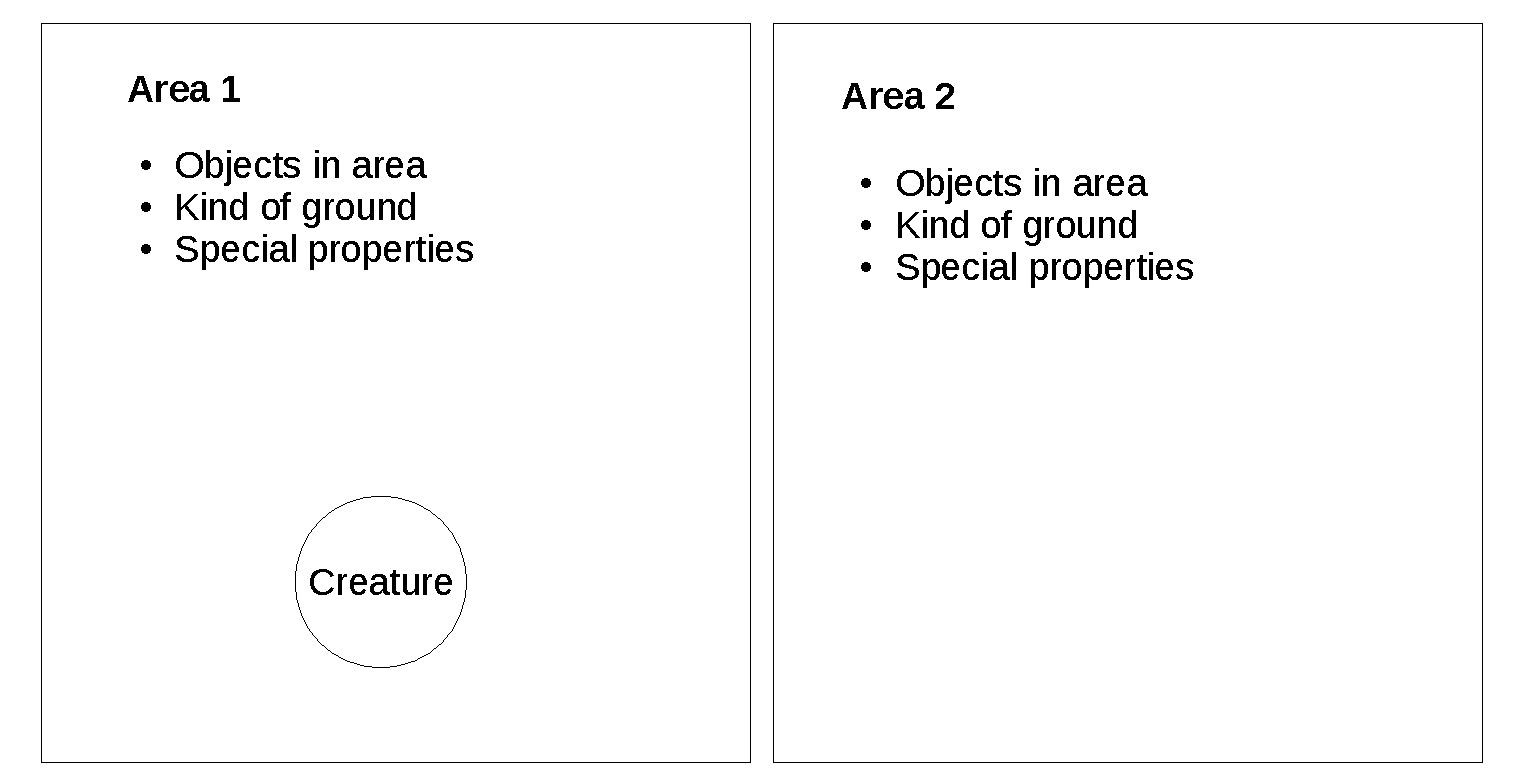
\includegraphics[scale=0.5]{combat0}

\subsection{Combat Areas}
In the diagram above we can see a basic schematic of a battle scenario, you can make these out of cardboard for your own games. It consists of two areas, here just called 1 and 2. Each area will obviously have a more descriptive name in an actual fight, and have actual properties detailed on it. The type of terrain should be noted so that players know how hard it is to move around the fight, and whether there are objects or circumstances they can take advantage of (like boulders they push down a hill, or a river they can knock enemies into). Creature tokens can be used to represent which players or enemies are currently in which area. Leaving a combat area that contains enemies results in a \textlf{Moment of weakness} (see Section~\ref{sec:aoo}).

\subsection{Distances and Radii}
A distance of 1 is size of 1 combat area (around 10 - 12 m in real life). In this system you measure a distance as the number of area boundaries crossed. So moving from one area to another is distance of 1. So to determine if an enemy is in range of a shooting attack you must count how many area borders the projectile must cross and compare it to the weapon range. A radius of 1 would cover a single area and ALL adjacent areas. An effect that is called \textlfirst{adjacent}, or radius 0, applies to a single combat area. 

\subsection{Basics of Movement}
Most creatures may transfer between combat areas, or move anywhere within one they are already in at the start of the turn, unless otherwise noted or modified by terrain. Movement actions cost 1 action point if the character wishes to change combat area. Normal movement in this manner is thus said to have a range of 1. 

\subsection{Basics of Attacks}
Attack-type actions represent making attempts to injure an enemy, they come in two varieties: ranged attacks, which are made with bows, guns, etc., and close-combat attacks which are made with swords, fists, etc. Successful attacks can batter the target, reducing its \textlf{endurance}. Once a creatures \textlf{endurance} is depleted it is exhausted, and further attacks can seriously injure it (this will detailed in the more advanced combat rules). A character can only make one attack per turn, unless otherwise modified. 

Declaring an attack costs 1 action point. During resolution the attacker and their target make an opposed check with \textlf{aim} and \textlf{deflect} respectively. If the attacker wins then the attack has struck home and moves on to roll damage checks.

\subsection{Close-Combat}
A character can make close-combat attacks against any creature within the same combat area as he is (range 0). The \textlf{aim proficiency} is for the \textlf{close-combat} skill.

\subsection{Ranged}
A character armed with a ranged weapon can often attack enemies that are in different combat areas to itself. How far it is allowed to do so is defined  by the weapon's range score. A range of 1 would allow shots to be fired at a target in any adjacent area to that of the firer. Draw a straight line between the shooter and target and count the number of area boundaries it passes over. The \textlf{aim proficiency} is for the \textlf{shooting} or \textlf{throwing} skill as appropriate.

\subsection{All-out attack}
The character channels all their energy into aggression. This attack action can be made with any kind of weapon, it costs 2 action points but grants an extra damage roll (from one of the character's weapons if wielding two). This cannot be used with weapons that have a \textlf{reload} rule.


\section{Combat - More Details}

\subsection{Moment of Weakness}
\label{sec:aoo}
These are moments when an opponent opens his guard or shows vulnerability, allowing an attacker to strike unhindered. A creature subject to a \textlf{moment of weakness} suffers an immediate damage roll from one enemy within reach (radius 0 for human-sized creatures). Sometimes the enemy who may exploit the free hit is specified by the effect, otherwise the fastest eligible enemy gets the hit.
Each creature or player can make only one of this type of attack per round. 

\subsection{Changing weapons}
To swap their current held the weapon a character must spend 1 action point and suffers a \textlf{moment of weakness}.

\subsection{Other Types of Movement}
\subsubsection{Running}
A character can run, at a cost of 2 action points, he then adds 1 to his movement range and he an \textlf{edge} bonus on \textlf{deflect} checks for 1 round. 

\subsubsection{Retreat}
At a cost of two action points the character can make a normal move, while leaving an area occupied by enemies, and not suffer any moment of weakness.

\subsection{Attacks that Hit}
If an attacker lands a successful attack on his foe, as described above, he may then make a damage roll to see if his blow injures the target. 

\subsubsection{Multiple Weapons}
If the character is using a weapon in each hand, he may attack with both for 1 action point. Only one opposed \textlf{deflect} vs \textlf{aim} check is made, but, each weapon gets separate damage rolls. Unless the character has the \textlf{Two-Weapon Fighting} \textlf{perk} (or other special rule) he suffers a \textlf{aim} \textlf{edge} penalty on such attacks.

\subsubsection{Damage Rolls}
\label{sec:dmg}
This represents whether or not a telling blow penetrates your target's armour.

A damage roll is a \textlf{power} check with the victim's \textlf{toughness} as \textlf{difficulty}. If the check succeeds then the victim loses \textlf{endurance} and, after reaching zero, collects wound cards to track how much of a potentially lethal battering they have suffered. See Section~\ref{sec:wounding} for the effects of any damage inflicted in this way (or below for the basics).

\subsubsection{Basics of Damage}
If a character suffers a hit he loses \textlf{endurance} points. How many are lost depends on the \textlfirst{lethality} of the attack. The grades being normal, crushing, devastating, and vorpal. These remove 1,2,3, and 5 \textlf{endurance} points respectively. Once a character has no \textlf{endurance} left, further damage is accumulated as actual injuries which are tracked via \textlf{wound} cards. 

Against targets with zero \textlf{endurance}, an attack of normal lethality will just wound its victims (dealing a \textlf{wounded} card), whereas crushing lethality inflicts the \textlf{badly-wounded} state with appropriate card, and \textlf{devastating} adds a second \textlf{badly-wounded} card. Vorpal attacks deal a \textlf{mortally-wounded} card to their victim.
If a character is \textlf{wounded} (i.e. he has a face up `wounded' card) they suffer an instance of the \textlf{Staggered} effect. Very serious damage is referred to as \textlfirst{badly wounded}, which inflicts an \textlf{edge} penalty on all the victim's rolls while the \textlf{badly-wounded} card is face up. \textlfirst{Mortally wounded} characters will die if they do not receive medical attention and cannot make any strenuous actions. 


\subsection{Additional Attack Rules}
\label{sec:close-combat}
\subsubsection{Critical Hits}
For every $\dicecritlvl$ a damage roll exceeds the victim's \textlf{toughness} by, the \textlf{lethality} of the attack is upgraded by one level. This is to represent the effects of extremely telling blows.
%
%\subsubsection{Glancing Hits}
%If the victim's \textlf{deflect} check scores equal to the \textlf{difficulty} then the attack is a \textlfirst{glancing hit}, causing the attacker to suffer a re-roll penalty to his damage rolls. 

\subsubsection{Penetrating Hits} 
If the target of an attack loses the opposed \textlf{aim}/\textlf{deflect} check by $\dicecritlvl$ or more then the attacker has achieved a \textlfirst{penetrating hit}, this allows associated damage rolls to gain one \textlf{edge} bonus per critical success threshold on subsequent damage rolls. 

\subsubsection{Ranged Weapons}
These are divided into two classes, this division determines how your aim is calculated. As with close combat targets, make one opposed \textlf{aim}/\textlf{deflect} check only against a given victim. If the attack has multiple projectiles you simply make the appropriate number of damage rolls.

First is shooting weapons: this subset encompasses bows, crossbows, and fire-arms. These weapons are operated to mechanically fire an arrow or similar projectile, requiring less exertion to use than it would to throw the projectile yourself. These use shooting skill to determine your aim score. Shooting weapons suffer an \textlf{edge} penalty on \textlf{Aim} when used on targets within range 0.

Secondly there are throwing weapons: this subset includes all types that are thrown by the force of a character's own arms/legs/limbs. 
Thrown weapons cannot be thrown effectively at point blank range (range 0) unless they are small weapons (dagger-sized).
Small throwing weapons can be dual-wielded. Throwing two small projectiles from the same hand incurs an \textlf{edge} penalty to the thrower's \textlf{aim}.





\section{Combat Areas - Terrain}
\label{sec:terrain}
\subsection{Open Terrain}
Grass, sand, tiles, gentle slopes or terrain that offers otherwise firm-footing is open terrain. This confers no bonuses or penalties to movement over it. Some open terrain, such as sand and low hedges that can easily be stepped over, count as low difficulty terrain for horses or similar mounts (but still require a riding check).

\subsection{Rough Terrain}
\label{sec:rough-t}
Loose rocks, tree roots, rubble, tables and chairs, similar obstructions of about knee or waist height, or surfaces that are unstable/moving/irregular are \textlfirst{rough terrain}. Moving into or out of \textlf{rough terrain} costs 1 action point more than normal.

For characters riding or driving, moving in \textlf{rough terrain} requires a ride/drive check versus a \textlf{difficulty} (chosen by the GM) between 8 and 12 (depending on how rough the terrain is) to avoid being unseated or losing control. 

\subsection{Dangerous Terrain}
Marsh-land, fast-flowing water, quicksand, thin ice, brittle rock, pools of acid or hot mud; these sorts of things are \textlfirst{dangerous terrain}. Any character entering, occupying, or moving through this terrain takes a hit with \textlf{crushing lethality} that causes damage on a $\dicediffbase+$ regardless of \textlf{toughness}. \textlf{Rough terrain} movement restrictions apply here as well.

For characters riding or driving, \textlf{dangerous terrain} requires a riding/driving check versus a \textlf{difficulty} (chosen by the GM) between 11 and 16 to avoid being unseated and both rider and mount suffering a damage roll with \textlf{power} equal to the check \textlf{difficulty} and \textlf{crushing lethality}. 



\section{Combat Areas - Cover}
\label{sec:cover}
If a combat zone offers cover then any creature within the zone may claim a bonus to any deflect checks it makes. Cover is divided into three categories and examples will be given below.
\begin{table}[ht]
	\centering
	\caption{Cover Table}
	\label{tab:cover}
	\begin{tabular}{|l|l|l|}
		\hline
		Cover Type & Deflect Bonus & Hide Bonus\\ [0.5ex]
		\hline
		Soft & - & \textlf{edge}\\
		Medium & \textlf{edge} & \textlf{edge}\\
		Heavy & 2$\times$\textlf{edge} & \textlf{edge}\\
		\hline
	\end{tabular}
\end{table}

\subsection{Soft Cover}
Good examples of soft cover are: small trees, bushes, wooden crates, soft furnishings and other such items that provide little protection but may conceal you from your enemies, and so, grant an \textlf{edge} bonus on any rolls to hide in them. Objects that provide soft cover can be broken with a \textlf{might}/\textlf{power} check against \textlf{difficulty} 6-9.

\subsection{Medium Cover}
Sandbags, hedges, low walls, small rocks, solid furniture. These kind of things provide a moderate amount of protection and concealment from enemies and an \textlf{edge} bonus to rolls to hide in the cover. Objects that provide medium cover can be broken with a \textlf{might}/\textlf{power} check against \textlf{difficulty} 9-13.

\subsection{Heavy Cover}
Battlements, Large walls, trees, big rocks, barricades, serious furniture (made of stone or steel). These things are built to provide a lot of cover and protection and also grant an \textlf{edge} bonus to rolls to hide in the cover. Objects that provide heavy cover can be broken with a \textlf{might}/\textlf{power} check against \textlf{difficulty} 13-20.


\section{Combat Areas - Examples}

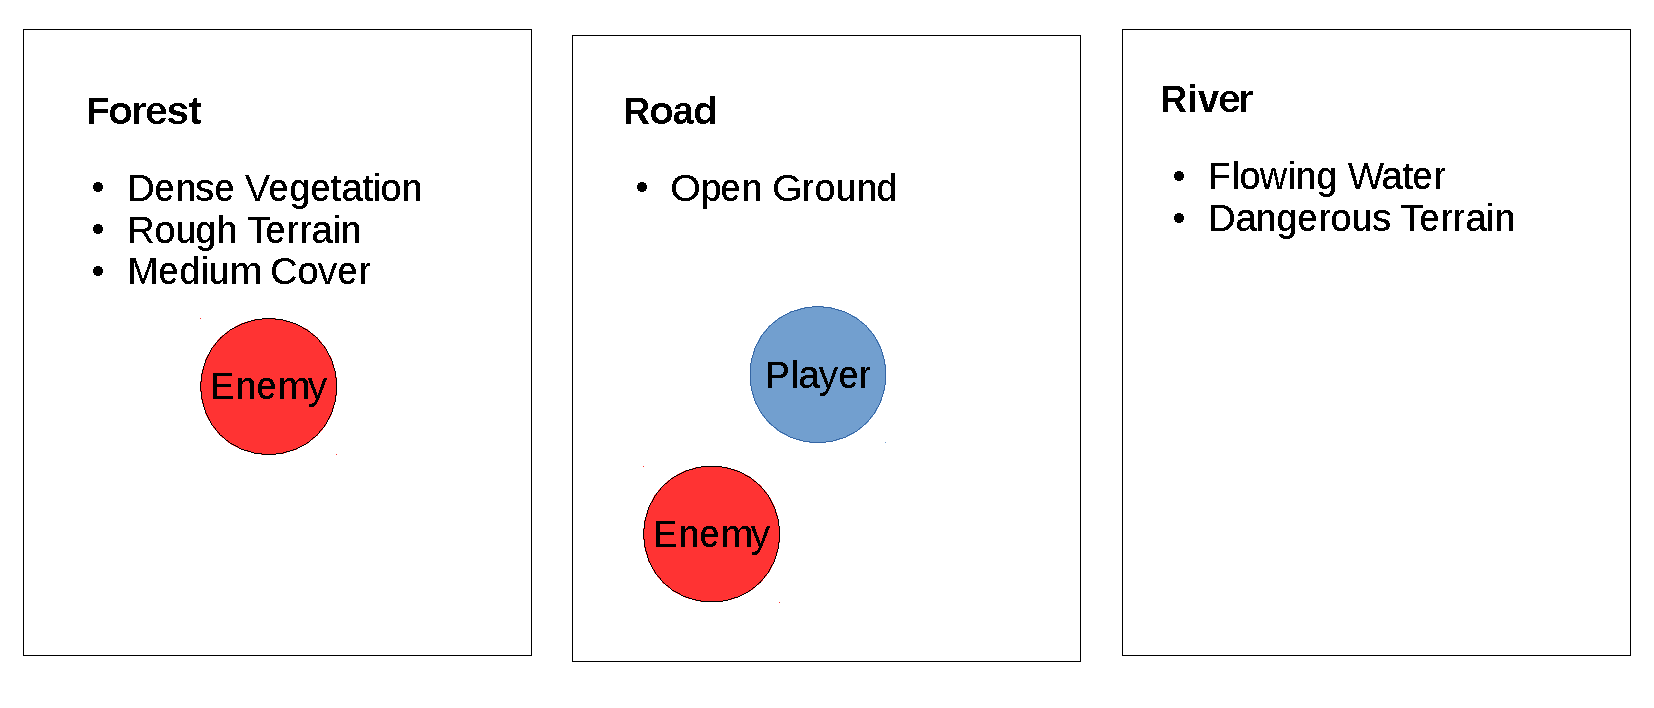
\includegraphics[scale=0.5]{combat1}


In our first example we see a fight with three combat areas. We can see it also has three participants, one player character and two enemies attacking him. The first area is the forest, which is \textlf{rough terrain} and provides medium cover. The road is open ground that confers no effects. Finally there is a river which is fast-flowing and thus \textlf{dangerous terrain}. We can see that in the road the player and enemy will be able to attack each other with any weapons. While the baddy hiding in the forest will be able to claim a cover bonus but will need a range 1 weapon to strike at the player.


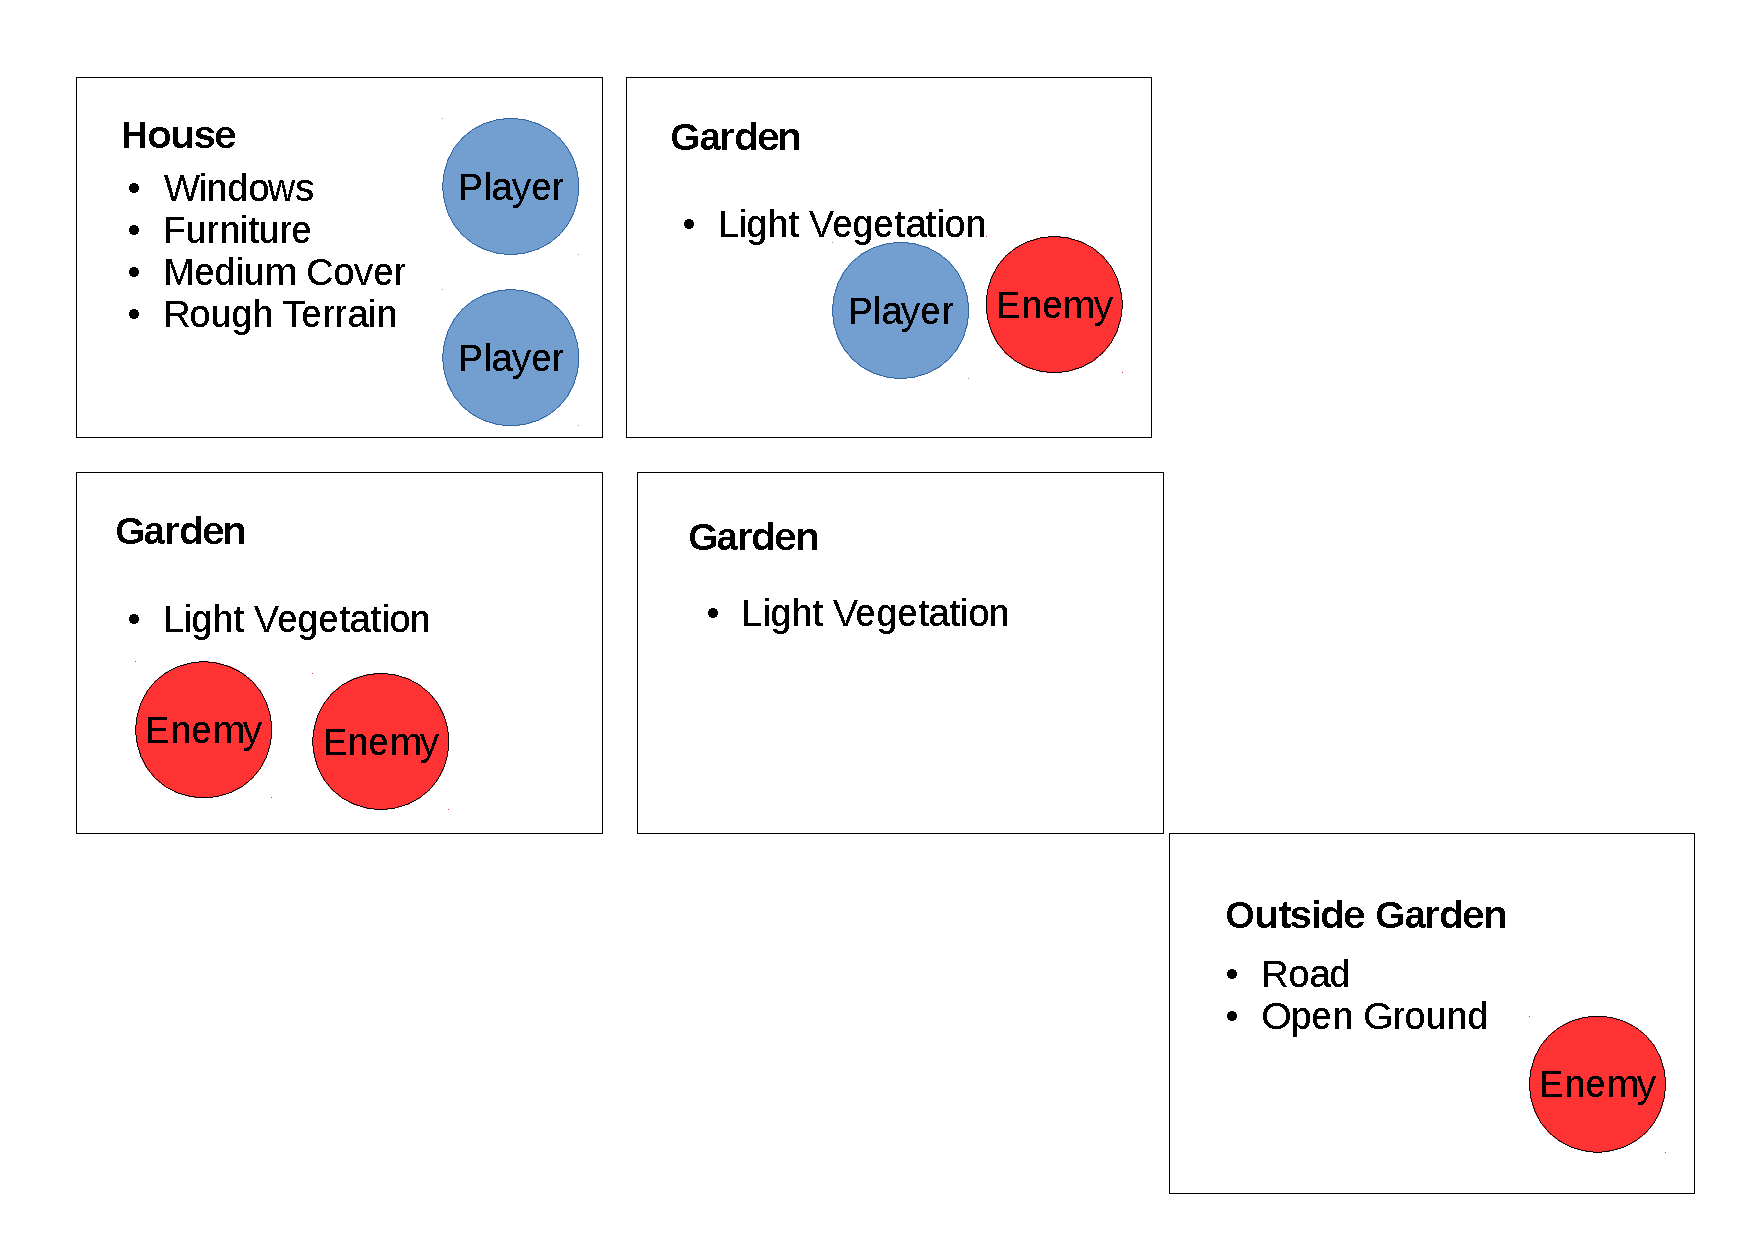
\includegraphics[scale=0.5]{combat2}

Our second example has a far more complex layout consisting of 5 areas. One is a house occupied by two player characters. The house provides medium cover to its occupants and they can attack out of the windows. Additionally, because it is a good defensive position it is labelled \textlf{rough terrain}, so enemies have difficulty moving into/through it. The garden has no special effect on combat and neither does the distant road. The players in the house will need range 1 weapons to hit the foes in the garden and range 2 to target the one out on the road. The player and enemy within one garden block can engage in either close-combat or fire ranged weapons at each other.



\section{Taking Damage and Wounding} 
\label{sec:wounding}
If a damage roll is successful against a creature then it either loses \textlf{endurance} or, when at zero, suffers a wound. How dangerous an attack is depends on the \textlf{lethality} of the weapon. Refer to Table~\ref{tab:lethal} and to the details in the sections below. If a character would be reduced to negative \textlf{endurance}, the lost points beyond zero are converted to wounds (i.e. -1 to \textlf{wounded} or -2 to \textlf{badly-wounded} etc).

\begin{table}[htbp]
	\centering
	\caption{Lethality Table}
	\label{tab:lethal}
	\begin{tabular}{|l|l|l|}
		\hline
		Lethality & Endurance loss & Wound \\
		\hline
		Normal & 1 & Wounded \\
		Crushing & 2 & Badly wounded \\
		Devastating & 3 & 2$\times$ Badly Wounded \\
		Vorpal & 5 & Mortally Wounded\\
		\hline
	\end{tabular}
\end{table} 

\subsection{Wounded}
Such a hit represents a flesh-wound and inflict an instance of the \textlf{staggered} effect on the victim. When the penalty expires the victim flips the card face down but keeps it to record the damage he has suffered.

A character with two face up \textlf{wounded} cards must exchange them for a \textlf{badly-wounded} card face up.

\subsection{Badly Wounded}
If a character suffers a wound from a weapon with \textlf{crushing lethality} he is dealt a \textlf{badly-wounded} card face up. While this is face up he suffers an \textlf{edge} penalty on all rolls. This card \textbf{will not} go face down automatically, it remains face up until remedied. Once face-down, the injury will heal within 10 days. 

The \textlf{devastating lethality} effect deals two face-up \textlf{badly-wounded} cards to the victim.  

A character with two face up \textlf{badly-wounded} cards is disabled, and cannot make actions.

\subsection{Mortally Wounded}
A \textlf{mortally-wounded} character cannot make actions and will die in three days unless he receives some medical attention. These cards cannot be flipped face down, only removed by healing.


\section{Recovery and Healing}
\textlf{endurance} is recovered completely if the character can rest for 8 hours. Otherwise, a short rest of around an hour restores 1 \textlf{endurance}.

A character that has suffered wounds can be healed via use of the Healing skill or by a non-player Healer. If the character has face-up wound cards, a roll is required every day. These rolls are made on 1d6 (if the wounds are at least washed and bandaged then use 2d6 and choose the lowest). If this roll is a 6, upgrade one \textlf{wounded} card to a \textlf{badly-wounded} card face up. Barring consequences of these rolls, a character passively heals one \textlf{wounded} card every 3 days and one \textlf{badly-wounded card} every 10 days.






\section{Situational Modifiers and Special Actions}
\label{sec:adv-spc}

\subsection{Light and darkness}
\label{sec:dark}
The lighting of an environment greatly influences the difficulty of fighting within it. There are three types of lighting: \textlfirst{full}, \textlfirst{low}, \textlfirst{dark}. \textlf{full} lighting has no effect, \textlf{low} incurs an \textlf{edge} penalty on \textlf{aim}, and \textlf{dark} means the character cannot see at all outside of 6 m (1 combat area) and also incurs \textlf{low} light penalties.

\subsection{Sneak Attacks}
\label{sec:sneak-attk}
A target that does not know of your presence, aggressive intent, or is otherwise fully engaged in combat with someone else (the target must have been unaware of your combat participation, if not your presence) is vulnerable to \textlfirst{sneak attacks}.

The victim of a \textlf{sneak attack} gets no opportunity to \textlf{deflect}, unless otherwise modified.
Such attacks always gain an \textlf{edge} bonus to damage rolls , and have \textlf{heavy weapon} 1 when made with \textlf{small} weapons, such as daggers, or with specialist tools, such as garrotte wire. Multiple \textlf{perks} can improve \textlf{sneak attacks}. \textlf{Small} weapon bonuses are lost on \textlf{Huge}, or larger, targets.

\subsection{Feints}
\label{sec:feint}
A feint costs one action point and requires an opposed cunning check with the target. Success allows you an \textlf{edge} bonus to \textlf{aim} this round, while failure results in a \textlf{moment of weakness} that can be exploited by the victim only. This has no effect with ranged weapons unless otherwise modified.

\subsection{Bull-rush}
\label{sec:bull}
This represents the character attempting to plough through enemies, knocking them down in the process. This costs 2 action points and is resolved as an opposed might check. The heavier participant gets an \textlf{edge} bonus on this check. If a character moved this turn he also gains an \textlf{edge} bonus. 

If the character using the \textlf{bull-rush} move wins, his target is knocked to ground. If the defender scores higher than the bull-rushing character, he is stopped in his tracks and suffers a \textlf{moment of weakness} exploitable by his target(s).

\subsection{Unarmed Attacks}
A character can attack his opponents with his fists and feet, or other appendages. Fighting unarmed against an armed foe results in a moment of weakness that any one target of your attacks that round may exploit. If a character has trained rigorously, his unarmed attacks are no longer subject to this penalty (\textlf{Unarmed Training perk}).

Unarmed characters may make a single punch/kick for 1 action point.

\subsection{Trip}
Attempt to entangle your foe's legs with your weapon's haft, or pointy bit built for tripping. Declare a \textlf{trip} attack before the \textlf{deflect} check is made. Should the attack land, it causes no damage roll but the target is \textlf{knocked down} (see Section~\ref{sec:special}) if it fails an opposed \textlf{Cunning} check. Weapons with the \textlf{Trip} rule can replace \textlf{Moment of Weakness} damage rolls with a \textlf{Trip} action instead.

\subsection{Disarm}
Even the mightiest warrior can be flummoxed by the loss of his precious sword.
Declare a \textlf{disarm} attack before the \textlf{deflect} check is made. Should the attack land, it causes no damage roll but renders the victim \textlf{vulnerable} (see Section~\ref{sec:special}) to the next damage roll if it fails an opposed \textlf{Might} check. Weapons with the \textlf{disarm} rule can replace \textlf{moment of weakness} damage rolls with a \textlf{disarm} action instead.

\subsection{Grapple}
You can attempt to wrestle your foe into an immobile state at the cost of 1 action point. Provided you have at least one free hand you make an opposed \textlf{Might} check with your target. If you win, the target is now \textlf{grappled}. However, if you lose you suffer a \textlf{moment of weakness} that can be exploited by the target. It costs 1 action point each round after the first to maintain a grapple.

\textlf{Grappled} foes cannot make any movement actions until they break free of the \textlf{grapple}, this costs 1 action point and requires that they win an opposed \textlf{Might} check with the grappler. If they are forced to move by some external effect then the grapple breaks automatically.

\subsection{Shove}
This costs 1 action point and involves an opposed \textlf{Might} check with the target, if the shover is successful the target is either knocked down or moved into an adjacent combat area (at the shover's discretion). Failure results in shoving character experiencing a \textlf{Moment of weakness}.

\subsection{Defensive stance}
This costs 1 action point and lasts 1 round. During this time the character gains an \textlf{edge} bonus to \textlf{deflect}.

\subsection{Prepared Actions}
\label{sec:prep}
A \textlfirst{prepared action} is one that the character does not wish to make immediately. Instead, he specifies the actions he wishes to make, as he would for a normal turn, but, in addition, specifies a condition for the activation of his prepared actions. Such as: he will make his actions in response to a specific action made by an enemy, or to an environmental event, like a wall collapsing. Having specified his prepared actions, the character then waits and executes his prepared action when the condition is met. If the condition is not met by beginning of the fighter's next turn, then the prepared action is not performed and the fighter may act as normal in his turn.

\subsection{Rage}
Many cultures hold that great warriors are capable of being consumed by a battle rage, indeed in the heat of battle, with adrenaline pounding through your veins, it is easy to simply let your instincts loose and lapse into a raging frenzy. In such a condition a warrior is legendarily hard to stop, he can suffer wounds that would kill a normal man and still continue to fight with unbridled savagery. However, this rage makes him reckless, as heedless of danger or injury he hurls himself into his enemies bringing death and destruction with him.

The mechanics below detail how this berserker fury affects characters and how they can initiate such a state.  

\subsubsection{Becoming Enraged}
A character becomes \textlfirst{enraged} if under extreme emotional strain while fighting, although particularly volatile personalities may become \textlf{enraged} more easily. Otherwise a character with the Berserker \textlf{power} can trigger an \textlf{enraged} state once per day.

\subsubsection{When Enraged}
An enraged character seeks to enter close combat with the nearest enemy at all times and cannot take prisoners, he goes only for the kill. If wielding a firearm type weapon, he may fire it at range (while moving as required). Enraged characters have an \textlf{edge} penalty on \textlf{deflect} checks and a lethality upgrade for their attacks.

Rage drains one point of \textlf{endurance} each round and ends when the character has no points left. A character cannot \textlf{enrage} unless they have at least one point of \textlf{endurance}. Damage rolls against an \textlf{enraged} target are made with an \textlf{edge} penalty.








\section{Enemies and Monsters}
\label{sec:monsters}
Enemies come in several categories, ranked according to their defining characteristics.

\subsection{Mundane Enemies}
These are generally creatures of humanoid or smaller size, this category is largely composed of humanoid soldiers, wolves or similar beasts.
\subsubsection{Abilities and Attributes}
Mundane enemies have no \textlf{heroism/villainy}, they can have \textlf{aim} bonuses ranging from 0-2, 0 being an inexperienced impromptu fighter and 2 being a well trained soldier. Such foes are likely to have zeros for most attributes, although the more experienced combatants may be suitably tougher and stronger (no attributes above 1 however). 
\subsubsection{Tactics}
These enemies are followers, they need to be lead. Without a leader to direct them, they are likely to be easily demoralised by powerful opponents or to simply attack the enemy they feel is the most threatening. Such behaviour is over-ridden in the presence of a leader. Mundane enemies must make a courage tests if they run out of \textlf{endurance} and if they suffer a \textlf{badly-wounded} effect, if they fail, they surrender or flee. Enemies who believe in their cause, or are mindless, are immune to this. When being lead, a mundane creature may use its leader's leadership score to make courage checks.

\subsection{Elite Enemies}
These are generally creatures who are extremely proficient combatants or are enhanced by some magical or technological power.
\subsubsection{Abilities and Attributes}
Such fighters are likely to have above average attributes, e.g. between one and three at levels 1 or 2. Elite enemies do not have any heroic attributes but may have multiple combat proficiencies.
\subsubsection{Tactics}
Such enemies are independent, they do not need to be lead, but are more effective with a leader to direct them. These foes are unlikely to be easily demoralised or intimidated by powerful opposition and will coordinate and work together to defeat stronger opponents. Elite enemies must make a courage test if they run out of \textlf{endurance} and if they suffer a \textlf{badly-wounded} effect, if they fail, they surrender or flee. Enemies who believe in their cause, or are \textlf{mindless}, are immune to this. When being lead, an elite creature may use its leader's leadership score to make courage checks.

\subsection{Enemy Leaders}
These are generally creatures who are proficient combatants but are also skilled at directing the actions of underlings.
\subsubsection{Abilities and Attributes}
Leader enemies are similar to elites in attributes but also have leadership proficiency.
\subsubsection{Tactics}
Such enemies co-ordinate their allies, using their leadership skill to enhance their fighting prowess and allowing lesser allies to adopt more sophisticated tactics. Leaders will attempt to avoid combat unless they are heavily reinforced. In other regards they behave similarly to elite enemies.

\subsection{Heroic Enemies}
These enemies are powerful heroes, much like the player-characters, except that they oppose the heroes for whatever reason that the GM decides should motivate them.
\subsubsection{Abilities and Attributes}
These enemies are individually as capable and powerful as player characters, sometimes more-so, and thus follow the same rules for heroic attributes and determining combat statistic scores. Heroic foes have attributes generated in a similar manner to players, although the Game Master may decide to give them more, or less, points to spend.
\subsubsection{Tactics}
Such enemies are leaders, they direct lesser foes in ways that will maximise their own advantage within a fight, they will also use their heroic attributes to the maximum possible effect. The presence of such enemies inspires and emboldens lesser enemies, making them less susceptible to intimidation and fear. Heroic enemies may surrender if they are severely injured or near death.

\subsection{Monsters}
These are enemies that are usually at least large creatures and often huge or titanic creatures (see Section~\ref{sec:special}). However, enemies that possess incredible supernatural powers or extreme natural abilities might fall into this field as well.
\subsubsection{Abilities and Attributes}
Such creatures have access to unique abilities or methods of fighting that might not need to depend on heroic attributes, monsters generally have low \textlf{aim} bonuses, as many monsters are large and have trouble making rapid manoeuvres. However, they have immense strength and aggression, larger creatures having high \textlf{power} to represent this. They may also, simultaneously, possess heroic attributes, but this is not needed, they are quite often mighty enough as it is. 
\subsubsection{Tactics}
These enemies are hugely dangerous and will simply exploit the powers, size or strengths that make them monsters in order to win. They attack enemies that seem the easiest prey, or those that otherwise attract their attention, unless they have the opportunity to get more than one foe at once. Some monsters may be extremely stupid, this limited intelligence can be exploited by players to distract or confuse such foes, such monsters may need a handler to direct them and counter-act their innate lack of quick wits. Monsters do not know the meaning of surrender or fear.


\section{Unnecessarily Advanced Combat Rules}

\subsection{Mounted Combat}
\label{sec:mountandblade}
Mounted combat is, as is quite obvious, combat while riding upon a mount. While mounted you gain the advantage of speed, mobility and the ability to trample your foes in addition to the devastating effects of a mounted charge.

\subsubsection{Mounted Charge}
Certain weapons, such as the lance and horse sword, utilise the power and speed of a mounted charge to the full, inflicting great damage as they smash into the hapless foe. This action costs 2 action points and allows a normal movement and attack action. The \textlf{difficulty} of the required ride check is 11 + 1 for rough and + 2 for \textlf{dangerous terrain} (with a possible dismount on failure). 

A mounted charge grants the rider an \textlf{edge} bonus to damage rolls this round.

\subsubsection{Trample}
You may attempt, while charging, to ride your opponent down and trample over him. This trample attempt requires a check opposing the mount's close-combat \textlf{aim} and victim's \textlf{deflect}. If the target wins he evades the trample, and you suffer a \textlf{moment of weakness} that the intended victim may exploit. However, if the \textlf{deflect} fails, the target is trampled beneath your mount's hooves/feet/wheels/appendages of motion. This results in the victim being knocked down and taking three hits which have \textlf{power} equal to that of the mount with an \textlf{edge} bonus. You cannot trample a target that is larger than you and your mount.



\section{Universal Special Rules}
\label{sec:special}
This is a collection of special rules that apply in all campaign settings and always mean the same thing regardless of context.


\subsection{Conditions}
These are negative statuses that a character can become subject to. 

\subsubsection{Vulnerable}
A powerful blow can sometimes open up a fighter to being easily finished off. All attacks directed at the victim benefit from an \textlf{edge} bonus to damage rolls for the effect's duration (default is 1 round).

\subsubsection{Staggered}
The shock of injury is a difficult thing to ignore and can incapacitate even the most hardened fighters. A \textlf{staggered} creature makes its next roll with an \textlf{edge} penalty. A character who has been subjected to X such effects faces the penalty on the next X rolls. 

%\subsubsection{Dazed}
%A \textlfirst{dazed} character has suffered a blow that leaves them with dizziness, blurred vision, or impaired judgement. Thus, such a character makes all \textlf{strike/aim} rolls with an \textlf{edge} penalty for 1 round.
%
%\subsubsection{Winded}
%A \textlfirst{winded} character has had the breath knocked out of them and suffers an \textlf{edge} penalty to his damage rolls for 1 round.

\subsubsection{Knocked Down}
A creature that is \textlfirst{knocked down} loses its footing and falls over. Such a creature is \textlf{vulnerable} until it can stand up. Standing up can be done only in your own turn. It costs no action points if the character wins an opposed \textlf{might} check with all adjacent opponents, otherwise it costs 1 action point.

\subsubsection{Blind}
A \textlfirst{blinded} creature has \textlf{aim} and \textlf{deflect} set to $-3$ for the duration of the effect and must randomise direction if it wishes to move.  

\subsubsection{Immobilised}
An \textlfirst{immobilised} creature cannot move, either due to some magical malaise or due to having suffered damage to its legs.

\subsubsection{Crippled}
The sudden shock of a well-placed blow can often neuter retaliation. If a \textlfirst{crippled} creature attempts to make attacks in its next turn these cost 1 more action point than normal. 

\subsubsection{Cursed}
A \textlfirst{cursed} creature is afflicted by a malignant magical effect sapping its luck and increasing the chance of misfortune. \textlf{Critical rolls} made by a \textlf{cursed} creature are treated as \textlf{critical failures}. \textlf{Curse} lasts until removed.

\subsubsection{Bleeding}
This state represents severe bleeding. 

\textlfirst{Bleeding} is a status that lasts 2 rounds, each round deal the victim loses 1 \textlf{endurance} or receives a \textlf{wounded} card face up. 

\subsubsection{Fear}
If a character is afflicted by this effect they must make a \textlf{resolve} check against a difficulty, chosen by the GM, based on how scary the situation is (a \textlf{heroism} point may be used to automatically pass). Should the character fail, they suffer an \textlf{edge} penalty on \textlf{aim} checks, each subsequent turn the character may try to pass the check again. 

\subsubsection{Terror}
If a character is afflicted by this effect they must make a \textlf{resolve} check against a difficulty, chosen by the GM, based on how scary the situation is (a \textlf{heroism} point may be used to automatically pass). Should the character fail, they must spend their each turn cowering in fear. Each subsequent turn the character may try to pass the check again. 

\subsubsection{Panic}
A non-hero creature may \textlfirst{panic} if it suffers considerable injury. If an elite or mundane enemy runs out of \textlf{endurance}, or is \textlf{badly-wounded}, it must make a \textlf{resolve} check vs \textlf{difficulty} 13. Should it fail, it flees or surrenders. In general, intelligent creatures will surrender, but this is up to the Game Master's choice. Note that the presence of a commander or leader will prevent weaker creature from giving up so easily, in this case the creature may use it's leader's leadership score for panic-related \textlf{resolve} checks.

\subsubsection{Poisoned}
Poisoned is a state that results from harmful chemicals being introduced into the victims system. A poisoned attack that injures a creature, poisons that creature if it fails a resolve check versus a \textlf{difficulty} associated with the virulence of the poison and the size of the dose. A \textlf{poisoned} character has one fewer action point in combat (to a minimum of 1) until cured of the poison.


%Table~\ref{tab:poison} reveals a few sample short action poisons suitable for use in combat. When applying poison to a weapon a character must make a perception check versus the poison's \textlf{difficulty} score or he accidentally applies a dose of the poison to himself. This can be avoided through the \textlf{Master Poisoner} expedient (Section~\ref{sec:expedients}).
%
%\begin{table}[ht!]
%\centering
%\caption{Poisons - D is the crafting \textlf{difficulty}, Potency is the power of the poison, Persistence is how many rounds of combat effects lasts, Cost is the ingredient cost, Alchemists will charge twice this for the product.}
%\label{tab:poison}
%\begin{tabular}{|l|l|l|l|l|}
%\hline
%Name & D & Potency & Persistence & Effect \\
%\hline
%Nightshade & 8 & 8 & 1 & Forfeit Next Action \\
%Paralysing Poison & 8 & 9 & 1 & Immobilised \\
%Soporific & 7 & 9 & 1 & Speed -2\\
%Neurotoxin & 11 & 10 & 2 & \textlf{edge} penalty: Deflect, Athletics\\
%Necrotic Poison & 13 & 11 & 2 & Crippled\\
%Widow Venom & 13 & 12 & - & Lethality upgrade\\
%Essence of Agony & 14 & 13 & 1 & Vulnerable\\
%\hline
%\end{tabular}
%\end{table}
%
%
%
%Poison for used in lethal doses for assassination tends to take longer to act but to be far more deadly. Such poisons will range in \textlf{difficulty} based on their virulence (doses do not apply in this case) and can range from acting within 10 minutes to several hours delay before the effects are felt. The resolve check to resist the poison is made in exactly the same way but success does not negate all the effects, the victim will still feel terribly unwell for several hours and be unable to undertake great physical exertion. Table~\ref{tab:long-poisons} has some sample lethal dose poisons
%\begin{table}
%\centering
%\caption{Lethal Dose Poisons - Delay is how long it takes to act, D is the crafting \textlf{difficulty}, Potency is the power of the poison, Cost is the ingredient cost, Alchemists will charge twice this for the product.}
%\label{tab:long-poisons}
%\begin{tabular}{|l|l|l|l|l|}
%\hline
%Name & Delay (mins) & D & Potency & Effect \\
%\hline
%Nightmare Draught & Till asleep & 9 & 9 & Horrific Nightmares \\
%Widow Venom & 15 & 13 & 10 & Death \\
%Arsenic & 120-360 & 9 & 11 & Death \\
%Scorpion Venom & 30 & 11 & 10 & Paralysis \\
%Mushrooms & 60 & 8 & 9 & Liver failure \\
%\hline
%\end{tabular}
%\end{table}



\subsection{Additional Attack Effects}

\subsubsection{Reach}
\textlfirst{Reach} represents the ability of close-combat weapons, like spears, to attack from a longer distance. A character with a \textlf{reach} weapon can make a free attack action each turn against a single enemy that enters his combat area, provided he is in \textlf{defensive stance}.

\subsubsection{Rending}
A well-placed blow from a \textlfirst{rending} weapon rips deep into the target. \textlf{Penetrating} hits from \textlf{rending} weapons benefit from a \textlf{lethality} upgrade.

\subsubsection{Massive Damage}
A weapon with \textlfirst{massive damage} does exactly as their name suggests. Thus, they have an \textlf{edge} bonus on their damage rolls, making mayhem all the more likely. An attack may benefit from multiple instances of this effect.

%\subsubsection{Crushing Blow}
%A Crushing Blow is an attack so forceful no mere flesh stands a chance. Consequently, such attacks have a Lethality upgrade as well as benefiting from the Massive damage rule. 

\subsubsection{Heavy Weapon X}
(X is an integer) A \textlf{heavy weapon} scythes through mortal flesh and bone with supreme ease, laying waste to all but the hardiest of creatures. Upon succeeding on a damage roll with such a weapon, the wielder may repeat the roll. These repeat rolls stop after X extra rolls or when a roll fails. Each time they succeeded on the extra rolls the \textlf{lethality} of the attack is upgraded. \textlf{critical success} on these rolls means a double \textlf{lethality} upgrade.

\subsubsection{Burst X}
(X is an integer) \textlfirst{Burst} represents attacks that explode, spray, splash, or carve into a wide area of flesh. An attack with \textlf{burst} X causes 1 + X damage rolls on a successful hit, rather than just one. 

\subsubsection{Penetration X}
(X is an integer) A weapon with \textlfirst{penetration} is designed to deal with heavily armoured opponents, sliding into weak-points or just inflicting blunt trauma through armour. Attacks from this weapon count the target's \textlf{toughness} as reduced by X, but cannot reduce it below $12$ in this way.

\subsubsection{Cleave X}
(X is an integer) An attack with \textlfirst{cleave} is one that can sweep in great arcs, cutting through many hapless foes with each swing. Such an attack may target up to X enemies at once. The attacker rolls once with his \textlf{aim} and each defender rolls with his \textlf{deflect}.



\subsection{Creature-Type Rules}

\subsubsection{Large Creature}
A creature is declared \textlf{large} if it exceeds 3 m in the main dimension (height, length,width depending on creature geometry). Thus, such creatures can only hide in medium or better cover but gain \textlf{cleave} 2 on all close-combat attacks. A \textlf{large} creature has an innate bonus of +1 \textlf{power}. Such a creature has 2 extra \textlf{endurance} points.

\subsubsection{Huge Creature}
Such vast beasts barely notice the damage inflicted by even the largest weapons a man can wield. In consequence they have 4 extra \textlf{endurance} points. Their colossal might means that these creatures also have \textlf{cleave} 3 on all close-combat attacks. \textlf{Huge} creatures have an innate bonus of +2 \textlf{power} and the size threshold to be declared \textlf{huge} is a requirement of least 6 m in the main dimension (height, length, or width depending on monster geometry). 

\subsubsection{Titanic Creature}
These behemoths are all but inured to the attacks of normal weaponry. In consequence they have 6 extra \textlf{endurance} points. \textlf{Titanic} creatures have \textlf{cleave} 4 on all close-combat attacks and \textlf{massive damage} against smaller targets. \textlf{Titanic} creatures have an innate bonus of +3 \textlf{power} and the size threshold to be declared \textlf{titanic} is a requirement of least 12 m in the main dimension (height, length, or width depending on monster geometry). Such beasts have range 1 on their close-combat attacks. 

\subsubsection{Small Creature}
Diminutive creatures are easily missed, even by the most vigilant of larger things. Consequently they get + 1 \textlf{deflect}.

\subsubsection{Mindless}
\textlfirst{Mindless} creatures have no thoughts, emotions, fear or creativity. Because of this, \textlf{mindless} creatures are immune to many occult powers, as well as not having to take \textlf{courage} checks. These creatures cannot use any advanced combat rules (no \textlf{flanking}, \textlf{sneak attacks} etc) apart from \textlf{grapple} and \textlf{bull-rush}.



\subsection{Weapons and Special Attacks}

\subsubsection{Dual-Wielding}
A character can wield a weapon in each hand if he so desires. While employing such armament the fighter makes only one \textlf{aim} roll, but a separate damage roll with each weapon if his attack hits. For weapons with \textlf{reload} rules, reloading takes 1 action point longer but both weapons are reloaded together. 

All characters dual-wielding have an \textlf{edge} penalty to \textlf{aim} without the \textlf{Two-Weapon Fighting perk}.

\subsubsection{Great-Weapons (GW)}  
Their weight and power grants the wielder the \textlf{massive damage} rule when striking his foe, but its size makes it unwieldy to the inexperienced. Great-weapons wielded by the untrained suffer an \textlf{edge} penalty to \textlf{aim}. This penalty is mitigated by the \textlf{Great-weapons perk}.

\subsubsection{Small}
\textlfirst{Small} weapons represent dagger-sized implements. These can used with great speed and easily concealed but tend to lack reach. Thus, they incur an \textlf{edge} penalty to close-combat \textlf{aim}. This penalty is negated against \textlf{Vulnerable} targets, during \textlf{sneak attacks}, or when paired with a larger weapon.






\chapter{Perks}
\label{chap:perks}
These are skills and talents learned or gained by a hero through the course of his adventures. They can be purchased through the expenditure of experience points with their cost given in brackets. Note that upgrades change their parent \textlf{perk}, they do not occupy a new \textlf{perk} slot.

\section{General proficiencies}
These perks do \textbf{not} occupy equipment slots for passive or active \textlf{perks}, their effect is always active.

\subsection{Great weapons (3)}
The character is no longer subject to an \textlf{edge} penalty on \textlf{aim} checks when he is wielding great-weapons.

\subsection{Heavy armour (3)}
(Requires \textlf{Medium armour}) The character has trained to use heavy armour effectively. This allows them to add their \textlf{resolve} (rather than $\dicenoprof$) to their \textlf{toughness} and negates the \textlf{deflect} penalty when wearing such armour.

\subsection{Instrument Proficiency: X (2)}
(Where X is a musical instrument type) The character has learned to play a chosen type of musical instrument (X) and no longer suffers the unknown-instrument penalties when playing this type of instrument.  

\subsection{Language: X (2)}
(X is a language) The character has complete fluency in the chosen language. 

\subsection{Master: X (7)}
(X must be a profession skill) The character has achieved mastery of his profession, his work is of unparalleled magnificence. Any crafting check for the mastered profession X an \textlf{edge} bonus.

\subsection{Medium armour (3)}
The character has trained to use medium armour effectively. This allows them to add their \textlf{resolve} (rather than $\dicenoprof$) to their \textlf{toughness} and negates the \textlf{deflect} penalty when wearing such armour.

\subsection{Skill proficiency: X (3)}
(Where X is a skill) The character is proficient with skill X, see Section~\ref{sec:skill-prof} for details.

\subsection{Two-Weapon Fighting (3)}
This allows the character to fight with two weapons simultaneously without an \textlf{edge} penalty on \textlf{aim} checks.

\subsection{Unarmed Training (3)}
The character has been tutored in the ways of fighting with fists and feet, he no longer suffers \textlf{moments of weakness} for fighting unarmed against armed foes.

\subsection{Unarmoured combat (3)}
The character has trained in the art of fighting without armour and knows how minimise the impact of attacks upon their flesh. This allows them to add their \textlf{resolve} to their \textlf{toughness} when wearing no armour.


\section{Active perks}
These open up new actions that a character can make and they must occupy an equipment slot for active \textlf{perks} to be usable.
\label{sec:active}

\subsection{Acrobatic Attack (4)}
(Requires \textlf{Acrobatic movement}). This costs 1 action point and allows the character to make both an \textlf{acrobatic movement} and attack action (against any target within range during the movement).

\subsection{Aimed shot (4)}
This action costs two action points and allows the character to make a single ranged attack with an \textlf{edge} bonus on \textlf{Aim} and associated damage rolls.

\subsection{Berserker (4)}
The character has harnessed his inner rage. This allows them to voluntarily \textlf{enrage} once per day.

\subsubsection{Upgrade: Towering rage (3)}
(Requires \textlf{berserker}) The character's rage is a terrifying sight as they plunge heedless into the foe. This grants the character an \textlf{edge} bonus to \textlf{aim}, but a similar penalty to \textlf{deflect}, while \textlf{enraged}.

\subsubsection{Upgrade: Berserkergang (4)}
(Requires \textlf{berserker}) The character has mastered their inner fury allowing them to Enrage twice per day.

\subsubsection{Upgrade: Endless rage (4)}
(Requires \textlf{berserker}) Becoming \textlf{enraged} restores the character's \textlf{endurance} to its maximum value. Additionally, the character can still become \textlf{enraged} when they have no \textlf{endurance} left.

\subsection{Best defence (4)}
When the character scores \textlf{critical success} on a \textlf{deflect} check their opponent suffers a \textlf{moment of weakness}. This can be used once per round.

\subsubsection{Upgrade: Unassailable (2)}
\textlf{Best defence} can be triggered once per round against each unique attacker.

\subsection{Blind Side (3)}
A deft feint allows the character enough room to fire his ranged weapons against close-combat assailants. When using a ranged weapon against a target within range 0 you may feint as though you were using a close-combat weapon. Success on the \textlf{feint} means you additionally ignore the normal \textlf{edge} penalty on shooting weapon hit rolls for targets within range 0.

\subsection{Butcher's blow (3)}
The force of the character's strikes cause them to inflict horrendous damage. This can declared when declaring an attack, the cost is increased by 1 action point. Should the attack cause damage, the target is subject to the \textlf{cripple} effect. This effect applies only to creatures a maximum of 1 size category larger than the character.

\subsection{Cleaving blow (4)}
This is an attack action that costs an additional action point but adds \textlf{Cleave} + 1 with any close-combat weapon that is wielded in two hands. 

\subsection{Deeds Not Words (4)}
Any time the character, or an ally within range 1, defeats a foe in combat the character may make a leadership action, that would otherwise cost 1 action point, for free. Defeat is defined by the enemy fleeing, surrendering, being incapacitated, or dying.

\subsection{Desperate Mechanisms (3)}
The character may reduce the \textlf{reload} action point costs of ranged weapons by 1. If he does so, he experiences an \textlf{edge} penalty on \textlf{aim} rolls.

\subsection{Diplomat (3)}
The character has great skill in pacifying angry or confrontational speakers, allowing him to do so with an opposed \textlf{resolve} check.

\subsection{Dragon Kick (2)}
(Requires Unarmed Training) The character may make an unarmed attack, after moving, in the form of a flying kick. This allows him to bypass intervening obstacles, and any such attacks that cause a wound also knock the target down. The knock down effect applies only to creatures a maximum of 1 size category larger than the character.

\subsection{Extra Sneaky (5)}
At a cost of 1 action point, the character's \textlf{sneak attacks} damage rolls gain a bonus level of \textlf{critical success} this turn.

\subsection{Flurry of Blows (3)}
A risky manoeuvre, the fighter replaces a considered attack with a hail of furious strikes. The character may declare they are making a flurry attack, in which case they may make an extra damage roll with a successful hit. However, the character suffers a - 2 penalty to their \textlf{aim} and \textlf{deflect} scores this round. This cannot be used if the weapon has the requirement of \textlf{reload} actions.


\subsubsection{Upgrade: Relentless (4)}
(Requires \textlf{Flurry of Blows}) The penalty associated with \textlf{Flurry of Blows} is reduced by 1.

\subsubsection{Upgrade: Barrage (3)}
(Requires \textlf{Flurry of Blows}) The character may use the \textlf{Flurry of Blows} effect as many times as he wants to each round, incurring the same bonuses each time but the penalty increases by a further -1 for each application of \textlf{Flurry of Blows}. Thus, making one bonus attack incurs a - 2 penalty to \textlf{aim} but a second bonus damage roll incurs an additional -3 penalty (-5 in total to attacks this round).

\subsection{Frothing fury (4)}
(Requires \textlf{berserker}) While \textlf{enraged} the character may spend 2 action points to make an \textlf{all-out attack} against all adjacent enemies. Additionally, this costs 1 \textlf{endurance} point.

\subsection{Guard breaker (3)}
This attack knocks the foe off balance. The character may declare this special attack for 1 action point. This inflicts no damage roll but causes the target to suffer an \textlf{edge} penalty on \textlf{deflect} and be \textlf{vulnerable} to the next attack action directed against it. 

\subsection{Intimidation (3)}
The character can intimidate a creature using their \textlf{persuasion} skill. This inflicts an \textlf{edge} penalty on the target's next roll of a type chosen by the character. In combat, this costs 1 action point.

\subsection{Iron Hand (3)}
The character's blows are capable of tossing his enemies aside like a child's toys. The character may declare an \textlf{Iron-Hand} attack before attempting close-combat attacks, in which case, his subsequent attack knocks the target up to a distance of range 1 in a chosen direction while also inducing a \textlf{knocked-down} state. The victim suffers no damage unless he collides with an obstacle (he enters \textlf{rough terrain} or cover). This effect applies only to creatures a maximum of 1 size category larger than the character.

\subsubsection{Upgrade: Fist of Steel (3)} 
(Requires Iron-Hand) As long as the character is unarmed, \textlf{Iron-Hand} attacks inflict damage in the same manner as normal unarmed attacks in addition to their special effects.

\subsection{Kick `em while they're down (5)}
At a cost of 1 action point, damaging \textlf{sneak attacks}, made in this turn, cause the victim to be afflicted with the \textlf{vulnerable} status.

\subsection{Lightning Fast (3)}
The character reacts so quickly that, during action declaration in combat, he may seize the initiative for his side at a cost of 1 action point. A character may not use \textlf{Lightning Fast} more than once per encounter (additionally, each side in combat can only benefit from this once per encounter).

\subsection{Martial Skill (3)}
At a cost of 1 action point the character's attacks this turn, with any close-combat weapon, count as having the \textlf{trip} and \textlf{disarm} rules. 

\subsection{Meteor Strike (2)}
(Requires Unarmed Training) The character gathers all his strength and makes a single unarmed attack, with only a single damage roll, this round. If he does so, this attack makes its victim \textlf{vulnerable} to the next damage roll it suffers.

\subsection{On the Hunt (5)}
The character may attempt to Hide while in combat for 1 action point, fading seamlessly into the background. Additionally all attacks made after hiding are \textlf{sneak attacks} but reveal the presence of the character. While hidden the character only incurs \textlf{moment of weakness} penalties if the potential attacker detects them.

\subsection{Pistol Whip (4)}
When using a ranged weapon that can be wielded in one hand the character may make a ``Pistol Whip" in place of a \textlf{sneak attack}. This is a close-combat attack that knocks the target down if it succeeds in causing a wound, if the victim fails \textlf{resolve} versus the \textlf{power} of the attack he is also rendered unconscious. This effect applies only to creatures a maximum of 1 size category larger than the character.

\subsection{Plan B (3)}
(Requires \textlf{Duelist}) Whenever one of the character's attacks is \textlf{deflected}, while in \textlf{Duelist} mode, he may make a free action where he draws and throws/fires a \textlf{small} throwing/ballistic weapon (this doesn't provoke a \textlf{moment of weakness}).

\subsection{Power attack (3)}
The character can declare a close-combat attack as a Power Attack. This makes it cost 1 extra action point but grants + 1 \textlf{power} on damage rolls. 

\subsubsection{Upgrade: Thews and sinews (2)}
(Requires \textlf{Power attack}) Power Attack also upgrades the \textlf{lethality} of associated damage rolls.

\subsection{Reckless strike (3)}
The character can declare a close-combat attack to be a Reckless Strike. Such an attack has an \textlf{edge} bonus to \textlf{aim} but the character incurs and \textlf{edge} penalty on \textlf{deflect} for one round.

\subsection{Splatter (3)}
The violence of your blows causes the blood of your foes to stain the soil. This can declared when declaring an attack, the cost is increased by 1 action point. Should the attack cause damage, the target is subject to the \textlf{bleeding} effect.

\subsection{Suppressing fire! (5)}
The character fires an indiscriminate volley of projectiles, forcing enemies and allies alike to get their heads down. This costs two action points, the character makes a ranged attack action against every creature (including allies) within a given combat area. All the targets gain an \textlf{edge} bonus to \textlf{Deflect}. This attack cannot be made with a weapon that requires action points be spent to reload it between shots.

\subsection{True Grit (3)}
Gritting their teeth the character keep fighting by sheer force of will. For 1 action point, the character can make a \textlf{resolve} check against 10 + the number of missing \textlf{endurance} points. On a success they regain 1 point of missing \textlf{endurance}.

\subsection{Upgrade: Savage Reprisal (2)}
(Requires \textlf{Adrenaline Rush}) Whenever the character triggers \textlf{Adrenaline Rush} he may make a single, free, close-combat damage roll against his assailant (provided he is within reach). This attack may also claim the benefit of the bonus granted by \textlf{Adrenaline Rush}.

\subsection{Whirlwind of steel (5)}
The character lashes out around him, striking all too slow to escape. This costs 2 action points and allows the character to make an attack action with their close-combat weapons against all adjacent enemies. 


\section{Passive perks}
\label{sec:perks}
These passively enhance the character and must occupy an equipment slot for passive \textlf{perks} to make their benefit usable.

\subsection{Made You Look (4)}
If the character succeeds on a \textlf{feint} action his subsequent attacks are \textlf{sneak attacks}.

\subsection{Might of heroes (6)}
Some warriors display such shear poise that they wield even the most awkward weapons with grace and skill. Your character can ignore the \textlf{cumbersome} rule.

\subsection{Weapon Specialisation: X (5)}
The character has trained long and hard in the use of a particular weapon type (X). As such, he gains an \textlf{edge} bonus on \textlf{aim} when wielding such a weapon proficiently. The available weapon types are setting specific and apply to broad categories (blunt weapons, pistols, etc). 

\subsection{Duelist (3)}
Fighting with a single weapon only, that does not require two-hands for effective use, allows for much more precise weapon control. Fighting in such a manner grants 1 bonus to \textlf{deflect}. Example: fighting with only a single rapier, or a longsword in only one hand (common theme is there is a free hand).

\subsubsection{Upgrade: Buckle Your Swash (2)}
(Requires \textlf{Duelist}) While fighting with a single weapon (as detailed in \textlf{Duelist}), the character may counter-attack once per round after succeeding on a \textlf{deflect} check.

\subsubsection{Upgrade: Or Swash His Buckle (2)}
(Requires \textlf{Buckle Your Swash}) The character may replace any \textlf{counter-attack} with a \textlf{disarm} attempt.

\subsection{Close quarters (3)}
The character is an expert at engaging at very close range with \textlf{small} weapons. This negates penalties associated with such weapons.

\subsection{Evasive (4)}
This grants + 1 \textlf{deflect}.

\subsubsection{Upgrade: Quick-Step (3)}
The character gains a + 1 bonus to \textlf{deflect} provided he doesn't wear heavy armour.

\subsection{Spontaneous Brawler (3)}
This allows the character to treat any weapon or improvised projectile as though it had the \textlf{throw} rule.   

\subsection{Leverage (4)}
\textlf{Trip} and \textlf{disarm} actions also \textlf{stagger} their victims.

\subsubsection{Roll with It (3)}
(Requires Unarmed Training) While wearing light or no armour the character may add his \textlf{perception} score to his \textlf{toughness}.

\subsection{Snake Fist (3)}
(Requires Unarmed Training) Unarmed attacks gain + 1 \textlf{power}.

\subsubsection{Upgrade: Tiger Claw (4)}
(Requires Unarmed Training \& Snake Fist) The character has learned to unleash a volley of strikes with hands and feet. Unarmed attacks make an extra damage roll. This does not incur \textlf{dual-wielding} penalties.

\subsection{Extension of Self (2)}
(Requires \textlf{Unarmed Training}) This extends the effects of \textlf{Snake Fist}, \textlf{Meteor Strike}, and \textlf{Dragon Kick} to quarter staves (or similar blunt martial arts weapons).

\subsection{Staff Mastery (4)}
The character may use a quarter staff (or other pole weapon) as though it was a dual-ended weapon, gaining an extra damage roll (with no weapon bonuses being applied to this). No \textlf{dual-wielding} penalties apply when using this \textlf{perk}.

\subsection{Professional wrestling (3)}
The character no longer suffers \textlf{moment of weakness} penalties associated with \textlf{Grapple} or \textlf{Shove} actions.

%\subsection{Warrior athlete (3)}
%The character can use \textlf{athletics} skill, instead of just \textlf{Might}, for \textlf{shove} and \textlf{grapple} actions.

\subsection{Eagle Eye (2)}
The character adds 1 to the range score of all ranged weapons he employs.

\subsection{Skirmisher (3)}
The character may use his close-combat proficiency for \textlf{aim} when firing ranged weapons at targets within range 0. When doing so he does not suffer an \textlf{edge} penalty on his hit rolls with shooting weapons.

\subsection{Always Carry a Spare (2)}
The character can produce a single extra dagger (or other \textlf{small} throwing weapon) in an emergency. This can be used at most once per day.

\subsection{Two in the Sleeve (4)}
Attacks with \textlf{small} throwing weapons allow two of them to be thrown from the same hand at no penalty. This adds an extra damage roll when such attacks hit their target.

\subsection{Bull-Headed (3)}
The character cannot suffer \textlf{moments of weakness} as a result of making a \textlf{bull-rush} manoeuvre (See Section~\ref{sec:bull}). 

\subsubsection{Upgrade: Stampede (3)}
(Requires Bull-Headed) The character may make a damage roll against one of the victims of their successful \textlf{bull-rush} actions. 

\subsubsection{Upgrade: Pain Train (4)}
(Requires Bull-Headed) The character may choose for his \textlf{bull-rush} to knock the target flying a distance of range 1, instead of just knocking it down. If the victim hits an obstacle (he enters \textlf{rough terrain} or cover) he suffers a damage roll, with \textlf{power} equal to the character's \textlf{might} and \textlf{normal lethality}.

\subsection{Adrenaline Rush (3)}
A surge of adrenaline can grant a fighter great power in times of danger. If the character loses \textlf{endurance} to a damage roll, they gain an \textlf{edge} bonus to their next damage roll.

\subsection{Executioner (3)}
The character has learned to deal death swiftly when the chance arises. As such, when striking a \textlf{badly wounded} opponent the character benefits from a \textlf{lethality} upgrade. This effect applies only to creatures a maximum of 1 size category larger than the character.

\subsection{Merciless (3)}
The character shows no mercy, dispatching the weak with even greater abandon. Attacks and spells against \textlf{bleeding} or \textlf{crippled} targets gain a \textlf{lethality} bonus on their damage rolls.

%\subsection{Mad Skillz (6)}
%Keep it comin'. Each time the character \textlf{critically hits} he may make an additional attack action against any chosen target. This cannot be recursively triggered, i.e. an attack generated by \textlf{Mad Skills} does not trigger this effect if it scores a \textlf{critical hit}.
%
%\subsection{Sudden Return (6)}
%When you start strong you have no choice but to push harder. If the character inflicts a \textlf{penetrating hit}, he may make an extra attack action against either the original target or one adjacent to it. This cannot be recursively triggered, i.e. an attack generated by \textlf{Sudden Return} does not trigger this effect if it scores a \textlf{penetrating hit}.

\subsection{Schadenfreude (3)}
The character gets an \textlf{edge} bonus to his next damage roll after inflicting \textlf{stagger} upon an enemy (see Section~\ref{sec:special}).

\subsection{Braced for Impact (4)}
The first time a character loses \textlf{endurance} each round, the amount lost is reduced by 1. 

\subsection{Indomitable (3)}
This allows the character an \textlf{edge} bonus on \textlf{resolve}-based checks against effects that would inflict \textlf{stagger}, \textlf{cripple}, \textlf{immobilise}, or \textlf{knock-down}.

\subsubsection{Upgrade: Stability (4)}
(Requires \textlf{Indomitable}) Inner strength is outer strength. Grants immunity to the \textlf{knock-down} and knock-back effects. If targeted by such an effect the character may still trigger \textlf{Juggernaut}.

\subsubsection{Upgrade: Juggernaut (3)}
(Requires \textlf{Indomitable}) This grants a free action point action after successfully passing a \textlf{Resolve}-based check against an effect that would inflict \textlf{stagger}, \textlf{cripple}, \textlf{immobilise}, or \textlf{knock-down}.

%\subsection{Determined (3)}
%Determined characters do not suffer an \textlf{edge} penalty on \textlf{deflect} when wearing \textlf{heavy armour}.

\subsection{Hardy (3)}
\textlf{Hardy} characters are mighty and indefatigable, they have an extra point of \textlf{endurance}.

\subsubsection{Upgrade: Stoic (4)}
(Requires \textlf{Hardy}) The character is so tough they can just ignore pain. This grants and additional point of \textlf{endurance}.

\subsection{On Guard (3)}
When the enemy strikes be prepared, when you strike be even more prepared. Every time the character \textlf{staggers} or \textlf{cripples} an enemy, they get an \textlf{edge} bonus on their next \textlf{deflect} check. 

\subsection{Fighting retreat (3)}
The retreat action now costs only a single action point.

\subsubsection{Upgrade: Rear-guard action (3)}
(Requires \textlf{Fighting retreat}). The benefits of \textlf{Fighting retreat} also apply to all allies adjacent to your character.

\subsection{Nimble (3)}
\textlfirst{Nimble} characters are quick and agile. Their movement actions have +1 range while wearing, at most, \textlf{light} armour.

\subsection{Acrobatic movement (3)}
The character can move out of, or through, a combat area containing enemies without suffering a \textlf{moment of weakness}. To do so they must win an opposed check with their \textlf{athletics} vs the highest \textlf{close-combat} skill enemy within the area in question. Failure on the check results in a \textlf{moment of weakness}.  

\subsection{Quick Draw (2)}
The character can change or draw weapons as a \textlf{free action} and is not subject to a \textlf{moment of weakness} for doing so. 

\subsubsection{Upgrade: Shoot First (3)}
(Requires \textlf{Quick Draw}) The character's attacks, made after making a surprise \textlf{Quick Draw} of \textlf{small} weapons (dagger or pistol sized) are \textlf{sneak attacks}. This bonus cannot be claimed outside the first round of (or prior to) a combat situation.

\subsection{Swift as Death (3)}
(Requires \textlf{Lightning Fast}) The character has an \textlf{edge} bonus on \textlf{aim} and \textlf{power} checks during a turn when he has triggered \textlf{Lightning fast}.

\subsection{Sixth Sense (3)}
The character is so sharp he can evade even unseen attacks at the very last minute. This allows the character to attempt to \textlf{deflect} \textlf{sneak attacks}, however, he does suffer an \textlf{edge} penalty on this.


%\subsection{Fast Learner (4)}
%(Requires \textlf{Reputation} level 5) A hero can pick up new skills with ease. Boost a chosen skill up to level 2.

%\subsection{Hero/Villain (0)}
%(Requires \textlf{Reputation} level 5) The character has become a hero, his praise is much sung, or his vile deeds whispered of, in local taverns. If the character has no \textlf{Heroism} remaining when he rests, he gains 2 points of \textlf{heroism} rather than 1.
%
%\subsubsection{Mighty Hero/Villain (0)}
%(Requires \textlf{Hero/Villain} and \textlf{Reputation} level 9) The character has become a figure of mighty stature and near mythical reputation, his acts of daring/honour/evil are known throughout the land. When resting, the character may always gain 1 point of \textlf{heroism}, regardless of how many he had before resting. 

\subsection{Crusader (5)}
When your ammunition is righteousness you seldom run out. Each time the character defeats an enemy he can regain a point of missing \textlf{endurance}. A defeated enemy is either: killed, knocked out, surrendering, or fleeing.

\subsection{Your mother was a hamster (3)}
The character has great knowledge of insults and is a master of taunting jibes. The character has an \textlf{edge} bonus on \textlf{resolve} checks intended to taunt or provoke a target into attacking them.

\subsection{Master Poisoner (3)}
The character has great knowledge of poisons and toxins. As such, he cannot accidentally poison himself while applying poison to a weapon.

\subsection{Favoured Environment: X (4)}
The character is skilled at moving and fighting in the chosen environment (X). This grants him an \textlf{edge} bonus to stealth, as well as survival checks while in this setting. The character is also not affected by \textlf{rough} or \textlf{dangerous terrain} associated with this environment.

\subsection{Favoured Enemy: X (4)}
The character is skilled in the killing of a chosen creature type (X). Against targets of type X  the character has an \textlf{edge} bonus on \textlf{aim}. X must be specific, ``humanoids" is too broad for instance, but ``humans" is fine in a cosmopolitan fantasy setting. If the setting is mostly human then ``human" is still too broad and it must be further narrowed down to a group, ``pirates" or ``ninjas" for instance.

\subsection{Cunning Plan (3)}\label{sec:sneak-expd}
When making \textlf{sneak attacks}, the character may use his \textlf{cunning} as the base statistic of his \textlf{power} (rather than his \textlf{might}, see Section~\ref{sec:comstat}).

\subsection{Low Blow (4)}
The character may also make \textlf{sneak attacks} against enemies who have any face-up \textlf{badly-wounded} cards, even if they don't meet any other pre-requisites for \textlf{sneak attacks} (see Section~\ref{sec:sneak-attk}).


\subsection{Seize the Advantage (4)}
The character may make \textlf{sneak attacks}(\ref{sec:sneak-attk}) versus foes who are \textlf{vulnerable}, even if they don't meet any other pre-requisites for \textlf{sneak attacks} (see Section~\ref{sec:sneak-attk}.

\subsection{Commanding Presence (6)}
Whenever the character succeeds on a leadership check an ally within range 0 of the character gains 1 point of missing \textlf{endurance}.

\subsection{Ballads of Battle (3)}
The character may use perform skill in place of leadership skill when making leadership actions, this requires that targets can hear the performance.


%\subsection{Skilful: X (3/6)}
%\label{expd:skilful}
%(X is a skill) The character gains an extra point to his skill proficiency. e.

\subsection{Moving Target (3)}
When mounted/driving and moving, the character has an \textlf{edge} bonus to \textlf{deflect} checks.

\subsection{Call in a Favour (2)}
(Requires Silver Spoon). The character can leverage his social connections to obtain a favour from a local noble, banker, crime-lord, warlord, or oligarch. This \textlf{perk} can only be chosen at character creation. 

\subsection{Pack Animal (2)}
(Requires Wanderer) The hunter brings his hunting companion wherever he goes. This grants him  a sympathetic animal companion that understands simple verbal commands and hand signals. The creature must be, at maximum, roughly equivalent to a dog in size and mass. \textlf{survival} checks can be made to get the animal to perform more complicated actions, like stealing a particular object, or distracting someone's attention. The creatures attributes are species specific. If you are proficient in \textlf{survival}, add 1 to all the combat statistics of your companion. This \textlf{perk} can only be chosen at character creation. A companion can be replaced, once dead, only at a cost of 5 experience. 

\begin{table}[ht!]
	\centering
	\begin{tabular}{|l|l|l|l|l|l|}
		\hline
		Creature & Might & Cunning & Perception & Resolve & Proficiencies \\
		\hline
		Canine & 0 & 0 & 1 & 1 & Close-combat, Survival \\
		Big cat & 1 & 1 & 0 & 0 & Close-combat, Sneak \& hide \\
		Bird & 0 & 1 & 1 & 0 & Close-combat, Awareness  \\
		Reptile & 1 & 0 & 0 & 1 & Close-combat, Sneak \& hide \\ 
		\hline
	\end{tabular}
\end{table}




\chapter{Baggage and Encumbrance}
\label{chap:loads}
Even a hero can only carry a limited amount of armour, weaponry, supplies, ladders, ropes, lanterns and the myriad of other things an adventurer might need. The Game Master need not police this too strongly, though don't let it get too silly. Some situations do call for some penalties, such a carrying a heavy pack while wearing heavy armour.

\section{Load Penalties}
Carrying too much around can make moving or fighting rather difficult. To reflect this, characters carrying a large back-pack, or wearing heavy armour, suffer an \textlf{edge} penalty to deflect checks.


\section{Carrying, Lifting \& Dragging Loads}
\label{sec:carry}
A character cannot carry more than a heavy load (40 kg + $2 \times$ \textlf{might}) for any real distance, but he can lift up to four times the weight of a heavy load, though only a few inches off the floor. A character can push or drag up to 6 times a heavy load on smooth surfaces but on rough or difficult ground he can push or drag only up to twice a heavy load. A character can lift any load lighter than twice his heavy load limit above his head. However these limits assume the character has lots of time to lift or move the heavy objects. If a character wishes to move or lift something rapidly he must make a \textlf{might} check, the \textlf{difficulty} is given by 7 for objects less than 15 kg, + 1 \textlf{difficulty} per additional 10 kg. If successful, a lifting check like this takes 1 action (3 seconds) to perform. For an object dragged via a might check, the \textlf{difficulty} is given by 8 for objects less than 30 kg, + 1 \textlf{difficulty} per additional 20 kg. Success allows the object to be dragged at the character's movement speed for two action points (6 seconds duration). 




%\section{Drunkenness and Intoxication}
%If a character sups too readily upon `stimulants' he may be become distinctly inebriated and lose some control of his actions. In order to represent this, if the Game Master decides a character is sufficiently intoxicated, he must roll his resolve score versus a \textlf{difficulty} that represents how drunk/intoxicated he is, these can be found on the table below. Should the test be failed, he must roll on the Drunk and Disorderly (or Tired and Emotional) Table~\ref{tab:drunk}. The margin of failure on the resolve check is added to the roll, any score below $\dicemin$ counts as $\dicemin$.
%
%\begin{table}[ht!]
%\begin{minipage}{0.4\textwidth}
%\centering
%\caption{Intoxication Table}
%\label{tab:intox}
%\begin{tabular}{|l|l|}
%\hline
%How Drunk? & \textlf{Difficulty} Score\\
%\hline
%Tipsy & 6\\
%Inebriated & 8\\
%Drunk & 10\\
%Plastered & 12\\
%Wasted & 14\\
%\hline
%\end{tabular}
%\end{minipage}
%\begin{minipage}{0.6\textwidth}
%\centering
%\caption{Drunk and Disorderly or perhaps `Tired and Emotional'?}
%\label{tab:drunk}
%\begin{tabular}{|l|l|l|}
%\hline
%Score & Intoxication \textlf{Difficulty} $<$ 10 & \textlf{Difficulty} $\geq$ 10\\
%\hline
%4-7 & Unsteady & Pass Out\\
%8-11 & Feel Sick & Vomit \\
%12-15 & Giggle Wildly & Burst into Song \\
%16+ & Get Aggressive & Offer Violence \\
%\hline
%\end{tabular}
%\end{minipage}
%\end{table}

\listoftables



\end{document}